\documentclass{cslthse-msc}
\usepackage[utf8]{inputenc}
\usepackage[english]{babel}
\usepackage{amsmath}
\usepackage{amsfonts}
\usepackage{amssymb}
\usepackage{amsthm}
\usepackage{breqn}
%\usepackage{makeidx}
\usepackage{graphicx}
\usepackage{framed}
\usepackage{tikz}
\usetikzlibrary{calc, shapes, backgrounds, positioning, matrix, shapes.multipart}
\usepackage{standalone}
\usepackage[titletoc, header, page]{appendix}
\usepackage{pdflscape}
\usepackage{hyperref}
\usepackage{mdwlist}
\usepackage{multirow}

%\geometry{showframe}

\author{
	Tommy Kvant \\
	{\normalsize \href{mailto:ada09tkv@student.lu.se}{\texttt{ada09tkv@student.lu.se}}}
}

\title{Task scheduling of multiple industrial robots through constraint programming}

\supervisor{Jacek Malec, \href{mailto:jacek.malek@cs.lth.se}{\texttt{jacek.malek@cs.lth.se}}}
\assSupervisor{Maj Stenmark, \href{mailto:maj.stenmark@cs.lth.se}{\texttt{maj.stenmark@cs.lth.se}}}
%\supervisor{Maj Stenmark, \href{mailto:maj.stenmark@cs.lth.se}{\texttt{maj.stenmark@cs.lth.se}}}
\examiner{Klas Nilsson, \href{mailto:klas.nilsson@cs.lth.se}{\texttt{klas.nilsson@cs.lth.se}}}

\acknowledgements{

}

\theabstract{

}

\keywords{key word}

\begin{document}
\makefrontmatter
\chapter{Introduction} 

\section{Background}
More and more of the production in today's society is getting automated. Manufacturers want to cut cost and make the production more effective by eliminating the human work and replace it with robots. But there are drawbacks; robots are expensive and robots does not have the versatility of a human. This puts pressure on the robot manufacturers to develop robots that are more versatile. Thus eliminating the need for manufacturers to have multiple robots to do multiple tasks and thereby lowering costs. And also by making the robots more versatile the close the gap of what a human and robots are able to do.

Current robot setups usually have one robot performing one task all the time, as oppose to flexible robots which will be performing many different tasks and assemblies. This poses the demand for the scheduling of such robots to be flexible as well. A scheduling of a robot can be a time consuming task. Since manufacturers want as effective assemblies as possible, it can take from days to weeks to perfect an assembly schedule. This is not feasible if you want to use the robot for many different tasks and assemblies. In this thesis we would like to try and automate this scheduling process in order to cut down on the scheduling time. To accomplish this we will be using Constraint programming, as it provides a general interface to solve problems without needing to build a complete framework from scratch. Also, scheduling is a classical constraint problem, thus constraint programming suits this problem well.

One of those robots are ABB's robot YuMi\textsuperscript\textregistered(formerly known as FRIDA). YuMi\textsuperscript\textregistered is a dual armed robot made to work along side humans and able to perform the some of the most complex tasks, such as mount a nut or thread a needle.\cite{_yumi_} It accomplishes this by using a wide variety of sensors, e.g. force sensor, visual sensors, etc. Usually robot replaces humans to perform dangerous or heavy tasks, YuMi\textsuperscript\textregistered is mainly designed for small parts assembly, i.e. usually humans roles in todays manufacturing environment.



\section{Project goal}
The goal of this thesis is to present a CP model suitable for a robot such as YuMi\textsuperscript\textregistered, able to handle the type of jobs YuMi\textsuperscript\textregistered is able to perform. It will be constructed using the MiniZinc language and tested using a couple of CP solvers and compare the results. Both to see how well our model can perform and how well the solvers perform relative to one another.

\section{Related work}
In Drobouchevitch et.al. 2006 they conclude that the increasing number of machines in a robotic cell causes an explosive growth in combinatorial possibilites. They also provide evidence that a dual-gripper cell is more productive than a single-gripper cell.\cite{sethi_2006}

Thörnblad et. al. 2009 concludes that when a cell is part of an assembly flow, the targeting of due dates instead of makespan is to prefer. The reason is that the focusing on makespan runs the risk of exacerbating an already unreliable flow.\cite{thornblad_2013} However, the assembly we perform is not a part of a flow, and thus we do not concern ourselves with maintaining a stable flow through the cell, but only to optimize the assembly in the cell.

Yuan and Xu 2013 states that constraint programming is only effective on small problems of flexible job shop scheduling. In order to effectively solve problems of larger size they suggest to use methods such as large neighbourhood search(LNS) or iterative flattening search. They also show that LNS together with Hybrid Harmonic Search produces good results.\cite{yuan_2013}
\\
Unfortunately MiniZinc does not support the implementation of custom searches such as LNS. Therefore we try to solve the problem of ineffectiveness by using filter such as them presented by Vilím in \cite{VilimBartak2002Batch} \cite{Vilim2002Precedence} and \cite{VilimBartak2002Sequence}.
\\\\
Unfortunately, not many comparisons between MiniZinc solvers where found. There is an annual competition held by NICTA where solvers can compete, this is the most comprehensive documentation of the performance of the solvers we have found. Unfortunately, they only present which solver wins a category and no statistics are presented. Hence, no deeper comparison can be made from the result. In the latest competition held, 2014, or-tools won three out of the four gold medals, Opturion CPX won all four silver medals and Choco won three out of the four bronze medals.\cite{mz_result_2014}

When presenting MiniZinc for the first time, initial tests was also presented comparing, amongst others, G12/FD, Gecode using FlatZinc code and native Gecode. The tests shows that MiniZinc was competitive with the native Gecode model and on average the Gecode front-end for FlatZinc was about 200ms faster than the G12/FD.\cite{mz_paper}

Another comparison found was done by Becket et. el. 2008 where they tested 10 solver on 12 problems. Unfortunately, the only solver tested there that we also used in this thesis is the G12/FD solver. So comparison with our results is hard. Although they did not draw any conclusions, G12/FD seem to fear relatively well compared to the other solvers tested.\cite{nicta_2964}


[ejenstam]\cite{ejenstam_2014}


\section{Report structure}

\chapter{Approach}

\section{Constraint Programming}
Constraint programing is a \emph{declarative} paradigm. This means that in contrast to \emph{imperative} paradigm languages, such as C or Java, the focus of solving problems using constraint programming is on specifying the solution and not the algorithm to solve it. This is done by specifying the solution using \emph{domain variables}, or simply variables, and \emph{constraints}. Variables have a domain of values, meaning they can represent each value in their domain. Variables can often be, depending on language and solver, either integers, floating-points, boolean or symbolic, symbolic being a text or label. For example a symbolic variable representing a week would have the domain\\
$\{Monday,Tuesday, Wednesday, Thursday, Friday, Saturday, Sunday\}$.

\subsection{Constraints}
Constraints are set up as relationships between the variables, and thereby limiting the domains of the variables. Integer domains are often used for variables, so for the rest of this section we will assume variables have integer domains. For this domain the following function symbols can be used: $+$, $\times$, $-$ and $\div$. The constraint relation symbols are $=$, $<$, $\leq$, $>$, $\geq$. Together with the function symbols and the constraint relation symbols, one can create simple constraint, called \emph{primitive constraints}. An example of a primitive constraint is $X < Y$, i.e.\ the values in $X$'s domain has to lower than in $Y$'s. Primitive constraints can be used to create more complex constraints using the conjunctive connective $\land$. An example of this is $X < Y \land Y < 10$, i.e.\ $Y$ has to be less than $10$ and $X$ has to be less than $Y$. Since all constraints has to hold when the model is evaluated, all constraints are joined in a conjunction.(\textbf{?}) The disjunctive connective $\lor$ is also available and can be used in the same way as $\land$. In some cases the logical implications; reverse implication ($\gets$), forward implication ($\to$) and bi-implication ($\leftrightarrow$) are also available. Here, for example, the implication works by taking two logical statement and if the first one evaluates to \emph{true} the other statement should hold as well. For example $X = 0 \to Y > 5$ says that if $X=0$ then $Y$ should be larger than $5$.

\begin{framed}
For example, we have a problem with the variables $x$ and $y$. $x = 4$ and $y = \{1..10\}$. Here the $x$ has the value $4$ and can thereby only assume the value $4$. $y$ on the other hand can assume the values $1$ to $10$. This means a solution to this problem can be $x = 4$ and $y = 1$ or likewise $x = 4$ and $y = 5$ , they are equally correct.\\
On this problem we can impose a constraint, for example $y > x$. Now we have set the constraint that $y$ needs to be larger than $x$. And since $x$ has a fixed known value we can directly see that $y > 4$, since $x = 4$. Now with this constraint, we can get rid of the lower part of $y$'s domain and now $y = \{5..10\}$ instead. And now a viable solution can be $x = 4$ and $y = 7$, but not $x = 4$ and $y = 3$.
\end{framed}

\begin{figure}
  \documentclass{standalone}
\usepackage{tikz}
\usetikzlibrary{calc, shapes, backgrounds}
\usepackage{standalone}
\usepackage{amsmath, amssymb}
\pagecolor{olive!50!yellow!50!white}
\begin{document}
\tikzset{
  leaf/.style = {draw=none,label = center:\textsf{$\vdots$}},
  labels/.style={midway, sloped, above, yshift=-10pt}
}
\begin{tikzpicture}
[
    scale = 0.75, transform shape, thick,
    every node/.style = {draw, circle, minimum size = 5mm, line width = 1pt, align=center},
    grow = down,  % alignment of characters
    level 1/.style = {sibling distance=6cm},
    level 2/.style = {sibling distance=2cm}, 
    level 3/.style = {sibling distance=1cm}, 
    level distance = 3 cm
  ]
 \node (Start){}
   child {   node [] (A) {}
     child { node [] (D) {}
       child { node [leaf] (M) {}}
       child { node [leaf] (N) {}}
     }
     child { node [] (E) {}
       child { node [leaf] (O) {}}
       child { node [leaf] (P) {}}
     }
     child { node [] (F) {}
       child { node [leaf] (Q) {}}
       child { node [leaf] (R) {}}
     }
   }
   child {   node [] (B) {}
     child { node [] (G) {}
       child { node [leaf] (S) {}}
       child { node [leaf] (T) {}}
     }
     child { node [] (H) {}
       child { node [leaf] (U) {}}
       child { node [leaf] (V) {}}
     }
     child { node [] (I) {}
       child { node [leaf] (X) {}}
       child { node [leaf] (Y) {}}
     }
   }
   child{ node(C){}
     child { node [] (J) {}
       child { node [leaf] (Z) {}}
       child { node [leaf] (A1) {}}
     }
     child { node [] (K) {}
       child { node [leaf] (B1) {}}
       child { node [leaf] (C1) {}}
     }
     child { node [] (L) {}
       child { node [leaf] (D1) {}}
       child { node [leaf] (E1) {}}
     }
   };

  
  % Labels
  \begin{scope}[nodes = {draw = none}]
    \path (Start) -- (A) node [labels] {Pick $X$};
    \path (Start) -- (B) node [labels] {Pick $Y$};
    \path (Start) -- (C) node [labels] {Pick $Z$};
    \path (A)     -- (D) node [labels] {$X=1$};
    \path (A)     -- (E) node [labels] {$X=3$};
    \path (A)     -- (F) node [labels] {$X=6$};
    \path (B)     -- (G) node [labels] {$Y=5$};
    \path (B)     -- (H) node [labels] {$Y=9$};
    \path (B)     -- (I) node [labels] {$Y=8$};
    \path (C)     -- (J) node [labels] {$Z=6$};
    \path (C)     -- (K) node [labels] {$Z=3$};
    \path (C)     -- (L) node [labels] {$Z=5$};
    \path (D)     -- (M) node [labels] {Pick $Y$};
    \path (D)     -- (N) node [labels] {Pick $Z$};
    \path (E)     -- (O) node [labels] {Pick $Y$};
    \path (E)     -- (P) node [labels] {Pick $Z$};
    \path (F)     -- (Q) node [labels] {Pick $Y$};
    \path (F)     -- (R) node [labels] {Pick $Z$};
    \path (G)     -- (S) node [labels] {Pick $X$};
    \path (G)     -- (T) node [labels] {Pick $Z$};
    \path (H)     -- (U) node [labels] {Pick $X$};
    \path (H)     -- (V) node [labels] {Pick $Z$};
    \path (I)     -- (X) node [labels] {Pick $X$};
    \path (I)     -- (Y) node [labels] {Pick $Z$};
    \path (J)     -- (Z) node [labels] {Pick $X$};
    \path (J)     -- (A1) node [labels] {Pick $Y$};
    \path (K)     -- (B1) node [labels] {Pick $X$};
    \path (K)     -- (C1) node [labels] {Pick $Y$};
    \path (L)     -- (D1) node [labels] {Pick $X$};
    \path (L)     -- (E1) node [labels] {Pick $Y$};   
  \end{scope}
\end{tikzpicture}
\end{document} 
%     without .tex extension
  % or use \input{mytikz}
  \caption{The beginning of the search space for the variables $X$, $Y$, $Z$, where $X=\{1,3,6\}$ $Y=\{5,9,8\}$ $Z=\{6,3,5\}$}
  \label{fig:search_space}
\end{figure}

\subsection{Global constraints}
\subsubsection{AllDifferent}
\subsubsection{Circuit}
\subsubsection{Cumulative}
\subsubsection{Global_Cardinality}



\subsection{Solver}
A constraint programming program is consisting of many of these constraints and variables. When the solution is specified in a model, a \emph{solver} runs the model. The goal of the solver is to satisfy all the constraints, i.e. set the domains of the variables so that the all follow the relationships of the constraints. This is called the \emph{constraint satisfaction problem}, and can  be defined as a triple $\langle Z,D,C \rangle$. $Z=\{x_1 \ldots x_n\}$ is a finite set of all the variables in the solution, $D(x_i), \; x_i \in Z$ is a set representing the domain of values the variable $x_i$ can assume, $C$ is the set of constraints imposed on the variables in $Z$. The solver accomplishes this by doing a \emph{search} on the space of possibilities, i.e.\ the \emph{search space}. The search space is in the form of a tree, where each branch is a selection of a variable where the variables domain is reduced into a smaller subset that conforms with the constraints. The solver traverses the tree in search for a solution. When all variables are set to conform with the constraints a solution is found. If the solver reaches a node where a variables domain becomes empty, it has to \emph{backtrack} to a previous node from which it can choose a new variable to set, i.e.\ traversing a new branch of that node.

\cite{tsang_1993}
\cite{marriott_1998}
\cite{mz_manual}

\subsection{Reified}

\section{Job-shop scheduling problem}
\subsection{Flexible job-shop scheduling problem}

\section{MiniZinc}
\section{Model}
This model is based on/inspired by the model in [ejenstam]. That model is centered around work performed in fixtures. So tasks can easily be labeled \emph{tray} if it uses a tray, \emph{fixture} if it uses a fixture, etc. This is common robot cell assembly procedures; take a component from a tray, put it in a fixture, get another component, mount the component on the the component in the fixture. But YuMi can perform much more complex tasks than that. We want to be able to schedule mounting tasks that does not incorporate a fixture. We have used a similar way of generalizing tasks by labeling them with \emph{tray}, \emph{fixture}, etc. but extended it.
\subsection{Input data}
The solver takes a description of the robot cell in the form of a MiniZink data file. The file describes; the number of arms available, the tools available, the trays available, the fixtures available, etc. Here on after called \emph{Cell Variables}. It also sets up a number of \emph{Decision Varibles} which contains a set of values from which each \emph{Decision Variable} can take.
\subsubsection{Cell Variables}


\subsubsection{Decision Variables}


\subsection{Constraints}
In this section some of the most important constraints for the model will be described. For a full list of used constraints see \emph{Appendix A}, for the MiniZink code see \emph{Appendix B}.


\subsection{Filter}
\subsubsection{Domain Filter}
\subsubsection{Predecessor Filter}

\section{Solvers}
\subsection{G12}
\subsection{JaCoP}
\subsection{Gecode}
\subsection{OR-tools}
\subsection{Opturion CPX}
\subsection{Choco3}
\chapter{Model}\label{cha:model}

 This model is inspired by Ejenstams work \cite{ejenstam_2014}. That model is centered around work performed in fixtures. So tasks can easily be labeled \emph{tray} if it uses a tray, \emph{fixture} if it uses a fixture, etc. This is common robot cell assembly procedures; take a component from a tray, put it in a fixture, get another component, mount the component on the the component in the fixture. But YuMi can perform much more complex tasks than that. We want to be able to schedule mounting tasks that does not incorporate a fixture. We have used a similar way of generalizing tasks by labeling them with \emph{tray}, \emph{fixture}, etc. but extended it.
 \\\\
Before going in to too much detail we will give a brief overview of how the scheduling works. We are working with tasks. A task is a action that manipulates a component in some way and is performed at a certain spacial coordinate in the room. Although, the model does not care about the exact coordinates, but rather the time it takes to travel between the coordinates. This time is used to establish how long the move from one task to the next will take. These moves are present for all tasks. If two tasks are performed at the same location, the move time will be $0$. The times needs to be calculated before hand and put in a matrix which is used to generate the input file for the model. How to do that is described in appendix \ref{cha:tool_manuals}.

The robots that the model schedules have arms, these we call machines. And no matter if the assembly has two one-armed robots or one two-armed robot, the number of machines are the same and will be scheduled the same. To compensate for the placement of the machines there are variables that can be set as shown below. The arms can have a set of tools that they can change between depending on what is required by the task. The change of a tool is incorporated in the move from one task to another. This is part of what the model will try to decide, where should we put the change of tools of the machines. If a change occurs between two tasks, it will be noted by the move taking longer than it usually would.

 The goal for the assembly is to assemble components. This is components fed to the assembly from the outside, for example button components. The final assembly is the complete assembly of components that make the final product. All the smaller assemblies before that are called sub-assemblies. For reasons explained further down, we will in this thesis call components such as buttons for \emph{primitve} components instead of just components.
\\\\
 All the data used by the model can be generated using the tools described in appendix \ref{cha:tool_manuals}.
 
 \section{Variables}
 The solver takes a description of the robot cell in the form of a MiniZinc data file. The file describes; the number of arms available, the tools available, the trays available, the fixtures available, etc. We will list all these in \emph{model variables} and then they will be explained further down among the \emph{static variables}.
 
 \subsection{Model Variables}
\begin{itemize*}
\item $nbrTasks$
\item $nbrMachines$
\item $nbrTools$
\item $nbrTrays$
\item $nbrFixtures$
\item $nbrComponents$
\item $nbrOutputs$
\item $nbrConcurrentGroups$
\item $nbrOrderedGroups$
\item $tray_t$
\item $output_t$
\item $fixture_t$
\item $componentsUsed_t$
\item $mounting$
\item $taking$
\item $moving$
\item $putting$
\item $concurrentTasks_k$
\item $order_k$
\item $toolNeeded_t$
\item $changeToolDuration_{tool_1,tool_2}$
\item $duration_t$
\item $taskSubComponents_t$
\item $taskCompleteSubComponents_t$
\item $timeMatrix3D_{t1,t2}$
\end{itemize*}
 
 \subsection{Static variables}
 Static variables are variables that have a fixed value, or is a set or list containing fixed values.
 
 \begin{equation}\label{eq:1}
 nbrTasks \in \{1 , \ldots , 2^{32}-1\}
 \end{equation}
 \begin{equation}\label{eq:10}
 tasks = \{1 , \ldots , nbrTasks\}
 \end{equation}
 First we define the number of tasks to be scheduled. Each task is identified.

 \begin{equation}\label{eq:19}
 startTasks = \{nbrTasks+1 , \ldots , nbrTasks+nbrMachines\}
 \end{equation}
 \begin{equation}\label{eq:20}
 goalTasks = \{nbrTasks+nbrMachines+1 , \ldots , nbrTasks+nbrMachines \times 2\}
 \end{equation}
  As mentioned, this model is based on the technique of using predecessors to determine which task comes directly before another. This creates the need to have source and a sink node for each machine, we call them start tasks and goal tasks. As they are not provided as parameters, the model creates them and give them identifiers with numbers greater than the tasks to be scheduled. Each machine has to have a start task and a goal task. This means that there are as much start and goal tasks as there are machines. They are arranged such that first comes all the start tasks and then all the goal tasks. One can easily find the start task for a machine by $nbrTasks + m$, where $m$ is the machine in question. It is also easy to find the matching goal task by $nbrTask + m + nbrMachines$. If one thinks of the tasks, start and goal tasks as an array where the index is the number of the task, then it would look something like figure \ref{fig:tasks_array}.
  
\begin{figure}
	\centering
	\documentclass[border=4pt]{standalone}
\begin{document}

\sffamily
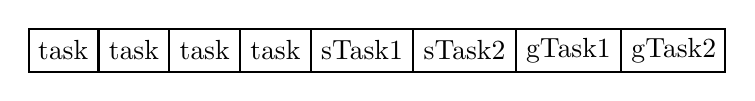
\begin{tikzpicture}[
  thick,
  myrect/.style={
    draw,
    rectangle split,
    rectangle split horizontal,
    rectangle split parts=#1,
    rectangle split part align=center
    } 
]

\node[myrect=8]
  {
  \nodepart{one}task
  \nodepart{two}task
  \nodepart{three}task
  \nodepart{four}task
  \nodepart{five}sTask1
  \nodepart{six}sTask2
  \nodepart{seven}gTask1
  \nodepart{eight}gTask2
  };

\end{tikzpicture}
\end{document}
	\caption{An example of the tasks and start and goal tasks seen as an array for an assembly with $4$ tasks and $2$ machines}
	\label{fig:tasks_array}
\end{figure}
 
 \begin{equation}\label{eq:21}
 allTasks = tasks \cup startTasks \cup goalTasks
 \end{equation}
 We group together all tasks in one set in order for a more readable notation further down.
 
 \begin{equation}\label{eq:2}
 nbrMachines \in \{1 , \ldots , 2^{32}-1\}
 \end{equation}
 \begin{equation}\label{eq:11}
 machines = \{1 , \ldots , nbrMachines\}
 \end{equation}
 Here we define the machines available for the assembly. A machine in this model is an arm.
 
 \begin{equation}\label{eq:3}
 nbrTools \in \{1 , \ldots , 2^{32}-1\}
 \end{equation}
 \begin{equation}\label{eq:12}
 tools = \{1 , \ldots , nbrTools\}
 \end{equation}
 \begin{equation}\label{eq:33}
 toolNeeded(t) \in tools, \; t \in tasks
 \end{equation} 
 These are the tools that can be fitted on an arm. The model assumes that there is a set of $nbrTools$ for each machine. I.e. if $nbrTools = 2$ and $nbrMachines = 2$, there is a set of tool $1$ and tool $2$ for machine $1$, and another set of tools $1$ and $2$ for machine $2$. There cannot be a combination of tools such as, for example, only tool $1$ for machine $1$ and a set of tools $1$ and $2$ for machine $2$.
 
 $toolNeeded(t)$ defines the tool task $t$ needs.
 
 \begin{equation}\label{eq:6}
 nbrComponents \in \{1 , \ldots , 2^{32}-1\}
 \end{equation}
 \begin{equation}\label{eq:13}
 components = \{1 , \ldots , nbrComponents\}
 \end{equation}
 \begin{equation}\label{eq:25}
 componentsUsed(t) \subset components, \; t \in tasks
 \end{equation}
 \begin{equation}\label{eq:componentCreated}
 componentCreated(t) \in components \cup \{0\}, \; t \in tasks
 \end{equation}
 $nbrComponents$ defines the number of components used. All components needs to be uniquely identified in the assembly, so even if we use 4 screws in an assembly, we need to define all 4 screws. As mentioned before we distinguish between components and \emph{primitve} components. The reason for that is that in the model we do not distinguish between a \emph{primitve} component and a sub-assembly, they are the same. And in the model we call them components. The reason for this is because we found it easier to only have one sort of object to deal with when it comes to what will be assembled, instead of two. This means that the final assembly is also a component, i.e. the product produced by the assembly is a component. In other words, in this thesis \emph{primitve} components and sub-assemblies are sub sets of components.
 
 $componentsUsed(t)$ defines the set of components task $t$ uses. A task usually only uses one component at a time, but uses two in the case of mounting tasks, the mounted component and the component mounted on.
 
 To know when a sub-assembly is created we set is as $compoentCreated$ for the task where it is created. This cannot happen anywhere else other than at a mount task, although there is no check in the model for it. If there is not component created at a task, $componentCreated=0$
 \\\\
 Since components also can be sub-assemblies, it means a component can have subcomponents. These have been grouped in different groups to assist the constraints.
 \begin{equation}\label{eq:53}
 taskSubComponents(t) \subset components, \; t \in tasks
 \end{equation}
 $taskSubComponents(t)$ is the set of components that make up the subcomponents for the components used in task $t$. One can think of the subcomponents as layers with the component on top, call it origin component, and the layer below are the components that make up that component, and so on. $taskSubComponents(t)$ contains the components one layer down, if the component itself is not a \emph{primitve} component. In that case, $taskSubComponents(t)$ contains that component instead.
 
 \begin{equation}\label{eq:54}
 taskCompleteSubComponents(t) \subset components, \; t \in tasks
 \end{equation}
 To use the layer metaphor again, $taskCompleteSubComponents(t)$ contains all the layers below the origin component, for all the components in task $t$. Not including the origin components themselves. If the origin component is a \emph{primitve} component, the set is empty.
 
 \begin{equation}\label{eq:55}
 subComponents(c) \subset components, \; c \in components
 \end{equation}
 $subComponents(c)$ contains only the the \emph{primitve} subcomponents for component $c$, one layer down. If $c$ is a \emph{primitve} component or is only made of sub-assemblies, the set is empty.
 
 \begin{equation}\label{eq:4}
 nbrTrays \in \{1 , \ldots , 2^{32}-1\}
 \end{equation}
 \begin{equation}\label{eq:14}
 trays = \{1 , \ldots , nbrTrays\}
 \end{equation}
 \begin{equation}\label{eq:22}
 tray(t) \in trays \cup \{0\}, \; t \in tasks
 \end{equation}
 The trays available in the assembly, $trays$. Trays are used to hold components until we need them in the assembly. This can be that the tray holds the components from the beginning, as with \emph{primitve} components fed to the assembly, or it can be a sub-assembly put there during the assembly to be picked up again later. Each \emph{primitve} component has its own tray, so we can have a button tray, a cover tray, etc.
 
 $tray(t)$ is the tray task $t$ uses. If no tray is used by the task, $tray(t) = 0$.
 
 
 \begin{equation}\label{eq:5}
 nbrFixtures \in \{1 , \ldots , 2^{32}-1\}
 \end{equation}
 \begin{equation}\label{eq:15}
 fixtures = \{1 , \ldots , nbrFixtures\}
 \end{equation}
 \begin{equation}\label{eq:24}
 fixture(t) \in fixtures \cup \{0\}, \; t \in tasks
 \end{equation}
 $fixtures$ defines the fixtures available in the assembly. A fixture is primarily used to hold a component in order for another component to be mounted on that component. Although, as will be shown in the assembly example [section?], the fixture can be used for purposes than just holding components.
 
 $fixture(t)$ is the fixture task $t$ uses. If no fixture is used by the task, $fixture(t) = 0$
 
 \begin{equation}\label{eq:7}
 nbrOutputs \in \{1 , \ldots , 2^{32}-1\}
 \end{equation}
 \begin{equation}\label{eq:16}
 outputs = \{1 , \ldots , nbrOutputs\}
 \end{equation}
 \begin{equation}\label{eq:23}
 output(t) \in outputs \cup \{0\}, \; t \in tasks
 \end{equation}
 $outputs$ defines the outputs available. An output is the final stage for a component in an assembly. After it is put here, it will not be removed. Although, there can still be other components mounted on the component put on the output. In that respect an output can be viewed as a fixture, only that the components put there can not be removed.
 
 $output(t)$ is the output used by task $t$. If no output is used by the task, $output(t) = 0$.
 
 
 \begin{equation}\label{eq:8}
 nbrConcurrentGroups \in \{1 , \ldots , 2^{32}-1\}
 \end{equation}
 \begin{equation}\label{eq:17}
 concurrentGroups = \{1 , \ldots , nbrConcurrentGroups\}
 \end{equation}
 \begin{equation}\label{eq:30}
 concurrentTasks(k) \subset tasks, \; k \in concurrentGroups
 \end{equation}
 $concurrentTasks(k)$ is the $k$:th concurrent group among the concurrent groups defined. A concurrent group is a group of tasks that has to be performed at the same time. Hence, a concurrent group can not be larger than the amount of machines available, although, there is no check for it in the model. 
 
 The $k$ set of tasks needing concurrent execution
 $nbrConcurrentGroups$ defines the number of concurrent groups used. 
 
 \begin{equation}\label{eq:9}
 nbrOrderedGroups \in \{1 , \ldots , 2^{32}-1\}
 \end{equation}
 \begin{equation}\label{eq:9}
 orderedGroups = \{1 , \ldots , nbrOrderedGroups\}
 \end{equation}
 \begin{equation}\label{eq:18}
 orderedGroup(k) \subset tasks, \; k \in orderedGroups
 \end{equation}
 \begin{equation}\label{eq:32}
 ordered(k,i) \in tasks, \; i \in \{1 , \ldots , |orderedGroup(k)|\}, \; k \in orderedGroups
 \end{equation}
 \begin{equation}\label{eq:39}
 orderedSet = \bigcup_{\forall k \in orderedGroups}order(k), \; orderedSet \subset tasks
 \end{equation}
 $orderedGroup(k)$ is the $k$:th ordered group specified, there are $nbrOrderedGroups$ ordered groups. An ordered group is an array of tasks that has to come in a very specific order. An example of this could be if an assembly has many move tasks that needs to be performed one after another in order to make an intricate movement. As will be showed in the constraints section, \ref{seq:constraints}, we can reason the relation between tasks if they use a certain component and are a certain kind of action. But we can not reason using two move tasks, there is no way to tell which should come before the other based on the component they use. 
 
 $orderedGroup(k)$ is an array and the tasks in it will be scheduled in the order they com in the array. All the tasks in the group will be performed on the same machine, it can not order tasks on different machines.
 
 If one wants to access a certain task in a group, one can use $ordered(k,i)$ to access the $i$:th element of the $k$:th group.
 
 $orderedSet$ is the set of all tasks included in an ordered group.
 \\\\
 $tray(t)$, $output(t)$ and $fixture(t)$ can not be set at the same time for a task, since that would mean the task is performed at two locations at the same time, although this is not checked by the model. The only restriction for what kind of tasks can be performed using these are that output can not be used by a take task and tray can not be used by a mount task. If ones assembly contains these combinations, the output or tray should be changed to a fixture.
 
 \begin{equation}\label{eq:26}
 mounting \subset tasks
 \end{equation}
 \begin{equation}\label{eq:27}
 taking \subset tasks
 \end{equation}
 \begin{equation}\label{eq:28}
 moving \subset tasks
 \end{equation}
 \begin{equation}\label{eq:29}
 putting \subset tasks
 \end{equation}
 Each task performed can be classified as either a mount task, a take task, a move task or a put task, but only one of them.
 \begin{description}
 \item[Taking] A task that picks up a component is a taking task. The location of the component is specified by either a tray or a fixture, but not an output since there is no reason to pick up something that has been placed on an output.
 
 \item[Mounting] A task that mounts a component on another component is a mounting task. This assumes that the component to mount is picked up and in the hand. The location of the component to mount on is defined by either a fixture or an output.
 
 \item[Putting] A task that puts a component somewhere is a putting task. Where a component is put is defined by either a fixture, a tray or an output.
 
 \item[Moving] A task that moves a components from one place to another is a moving task. The model already puts in moves between tasks and if, for example, the first task is a take task and the second task is a put task, the move in between them is essentially a move that moves a component from one place to the another. Although, sometimes it can be handy to define a task that explicitly moves a component. An example of that can be if one wants to spin a component around. Then one can specify a take task in order to pick up the component, a move task to turn it, and a put task to put the component back. In this case there will be three moves of the component; one to move from the take task to the move task, the move task itself, and a move from the move task to the put task.
 \end{description}
 \begin{equation}\label{eq:35}
 putting(c) \subset putting, \; c \in components
 \end{equation}
 \begin{equation}\label{eq:36}
 mounting(c) \subset mounting, \; c \in components
 \end{equation}
 \begin{equation}\label{eq:37}
 taking(c) \subset taking, \; c \in components
 \end{equation}
 \begin{equation}\label{eq:38}
 moving(c) \subset moving, \; c \in components
 \end{equation}
 $putting(c)$, $mounting(c)$, $taking(c)$ and $moving(c)$ are subsets of respective set above based on the component involved.
 
 \begin{equation}\label{eq:42}
 duration(t) \in \{0 , \ldots , 2^{32}-1\}, \; t \in tasks
 \end{equation}
 $duration(t)$ is simply the duration of task $t$.
 \\\\
   \begin{figure}
   	\centering
    	\documentclass{standalone}
\usepackage{tikz}
\usetikzlibrary{calc, shapes, backgrounds}
\usepackage{standalone}
\usepackage{amsmath, amssymb}
\pagecolor{olive!50!yellow!50!white}
\begin{document}

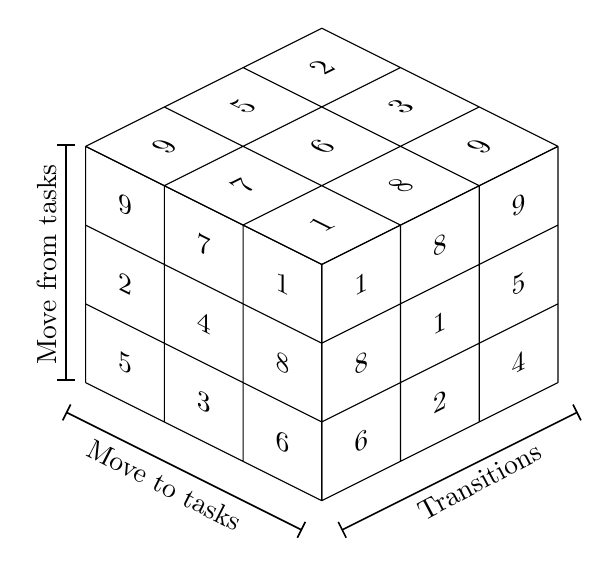
\begin{tikzpicture}
\begin{scope}[every node/.append style={yslant=-0.5},yslant=-0.5]
  \node at (0.5,2.5) {9};
  \node at (1.5,2.5) {7};
  \node at (2.5,2.5) {1};
  \node at (0.5,1.5) {2};
  \node at (1.5,1.5) {4};
  \node at (2.5,1.5) {8};
  \node at (0.5,0.5) {5};
  \node at (1.5,0.5) {3};
  \node at (2.5,0.5) {6};
  \draw (0,0) grid (3,3);
\end{scope}
\begin{scope}[every node/.append style={yslant=0.5},yslant=0.5]
  \node at (3.5,-0.5) {1};
  \node at (4.5,-0.5) {8};
  \node at (5.5,-0.5) {9};
  \node at (3.5,-1.5) {8};
  \node at (4.5,-1.5) {1};
  \node at (5.5,-1.5) {5};
  \node at (3.5,-2.5) {6};
  \node at (4.5,-2.5) {2};
  \node at (5.5,-2.5) {4};
  \draw (3,-3) grid (6,0);
\end{scope}
\begin{scope}[every node/.append style={
    yslant=0.5,xslant=-1},yslant=0.5,xslant=-1
  ]
  \node at (3.5,2.5) {9};
  \node at (3.5,1.5) {7};
  \node at (3.5,0.5) {1};
  \node at (4.5,2.5) {5};
  \node at (4.5,1.5) {6};
  \node at (4.5,0.5) {8};
  \node at (5.5,2.5) {2};
  \node at (5.5,1.5) {3};
  \node at (5.5,0.5) {9};
  \draw (3,0) grid (6,3);
\end{scope}

%x-axis
\draw[|-|,semithick,yslant=-0.5] (-0.25,-0.5) -- (2.75,-0.5);
\draw (1,-1.3) node[rotate= -27] {Move to tasks};

%y-axis
\draw[|-|,semithick,yslant=-0.5] (-0.25,-0.1) -- (-0.25,2.9);
\draw (-0.25,1.5) node[rotate=90, anchor= south] {Move from tasks};

%z-axis
\draw[|-|,semithick,yslant=-0.5] (3.25,-0.25) -- (6.25,2.75);
\draw (5,-1.25) node[rotate=28] {Transitions};
\end{tikzpicture}
\end{document} 

    	% or use \input{mytikz}
    	\caption{The timeMatrix3D}
    	\label{fig:3d_matrix}
   \end{figure}
 For the model to decide how long a move between two tasks should be and if there should be a change of tool in between, a matrix is used, $timeMatrix3D$, see figure \ref{fig:3d_matrix}. This is a 3-dimensional matrix and contains the times for moving between all the tasks depending on what tool change occurs. On its y-axis it has the tasks to move from, on the x-axis the tasks to move to, and on the z-axis the different transitions between tools that can occur.
 \begin{equation}\label{eq:timeMatrixDepth}
 timeMatrixDepth = \frac{n^2 - n + 2}{2}, \; n = nbrTools
 \end{equation}
  \begin{equation}
  \begin{aligned}\label{eq:44}
  timeMatrix3D(t(from),t(to),k) &\in \{0 , \ldots , 2^{32}-1\},\\
  t(from) &\in tasks \cup startTasks,  \\ 
  t(to) &\in tasks, \; k \in \{0 , \ldots , timeMatrixDepth\}
  \end{aligned}
  \end{equation}
 $timeMatrixDepth$ is the length of the z-axis, i.e. the depth of the matrix. It should be said that the reason for using the method described below is to reduce the size of the matrix and avoid too much redundancy.
 
 What we mean with ''different transitions'' is easiest to show through an example. Lets say we have $3$ tools available for each machine. We consider each tool state as a node in a graph, see figure \ref{fig:tools_trans_bef}, with the old tool state to the left and the new tool state to the right. Between them we can draw the different ways we can change state. The we start to consider which ones we actually need. We can change from tool $1$ to tool $1$, which is not changing tool at all. The same can be done for tool $2$, but not changing tool here costs just as much time as with tool $1$. So the change from tool $1$ to itself covers not changing tool for this tool, as well as for all the other tools, thereby we only need to keep track of one of these changes. We can also change from tool $1$ to tool $2$. And we can change back from $2$ to $1$, although here in the model we assume the change from one tool to another takes the same time the other way around as well. Therefore, we consider the change from tool $1$ to tool $2$ the same as from tool $2$ to tool $1$, and only keep track of one of them. If we keep consider the rest of the transitions this way, we will end up with a reduced number of transitions, in our case $4$, see figure \ref{fig:tools_trans_aft}
 
 It has been observed that using the reasoning above, $timeMatrixDepth$ follows the function \ref{eq:timeMatrixDepth}.
 
 \begin{figure}
 	\centering
 	\input{Figures/tool_trans_bef}
 	% or use \input{mytikz}
 	\caption{All the transitions between the tool states}
 	\label{fig:tools_trans_bef}
 \end{figure}
 
 \begin{figure}
 	\centering
  	\documentclass{standalone}
\usepackage{tikz}
\usetikzlibrary{calc, shapes, backgrounds}
\usepackage{standalone}
\usepackage{amsmath, amssymb}
\pagecolor{olive!50!yellow!50!white}
\begin{document}
\tikzset{
  leaf/.style = {draw=none,label = center:\textsf{$\vdots$}},
  labels/.style={midway, sloped, above, yshift=-10pt}
}
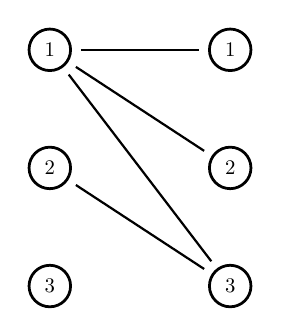
\begin{tikzpicture}
[
    scale = 0.75, transform shape, thick,
    every node/.style = {draw, circle, minimum size = 5mm, line width = 1pt, align=center},
    grow = down,  % alignment of characters
    level 1/.style = {sibling distance=6cm},
    level 2/.style = {sibling distance=2cm}, 
    level 3/.style = {sibling distance=1cm}, 
    level distance = 3 cm
  ]
  
  \tikzset{VertexStyle/.style = {shape          = circle,
                                   text           = black,
                                   inner sep      = 2pt,
                                   outer sep      = 5pt,
                                   minimum size   = 20pt}}
  \begin{scope}[node distance=20mm and 10mm]
  \node[VertexStyle](11){1};
  \node[VertexStyle, below of= 11](12){2};
  \node[VertexStyle, below of= 12](13){3};

  \node[VertexStyle, right= 2cm of 11](21){1};
  \node[VertexStyle, below of= 21](22){2};
  \node[VertexStyle, below of= 22](23){3};
  \end{scope}
  
  \draw(11) to (21);
  \draw(11) to (22);
  \draw(11) to (23);
  \draw(12) to (23);

% \node (Start){}
%   child {   node [] (A) {}
%     child { node [] (D) {}
%       child { node [leaf] (M) {}}
%       child { node [leaf] (N) {}}
%     }
%     child { node [] (E) {}
%       child { node [leaf] (O) {}}
%       child { node [leaf] (P) {}}
%     }
%     child { node [] (F) {}
%       child { node [leaf] (Q) {}}
%       child { node [leaf] (R) {}}
%     }
%   }
%   child {   node [] (B) {}
%     child { node [] (G) {}
%       child { node [leaf] (S) {}}
%       child { node [leaf] (T) {}}
%     }
%     child { node [] (H) {}
%       child { node [leaf] (U) {}}
%       child { node [leaf] (V) {}}
%     }
%     child { node [] (I) {}
%       child { node [leaf] (X) {}}
%       child { node [leaf] (Y) {}}
%     }
%   }
%   child{ node(C){}
%     child { node [] (J) {}
%       child { node [leaf] (Z) {}}
%       child { node [leaf] (A1) {}}
%     }
%     child { node [] (K) {}
%       child { node [leaf] (B1) {}}
%       child { node [leaf] (C1) {}}
%     }
%     child { node [] (L) {}
%       child { node [leaf] (D1) {}}
%       child { node [leaf] (E1) {}}
%     }
%   };
\end{tikzpicture}
\end{document} 

  	% or use \input{mytikz}
  	\caption{The reduced number of transitions between the tool states}
  	\label{fig:tools_trans_aft}
 \end{figure}
 
 \begin{equation}\label{eq:56}
 taskOutOfRange(m) \subset tasks, \; m \in machines
 \end{equation}
Depending on the physical layout of the assembly, sometimes not all tasks can be done with all machines. It could be that the machines would collide or simply that the spatial location is out of reach for the machine. In those cases we can specify tasks are out of hand for a specific machine. This is the only time when we distinguish between the two machines and connect the machine in the model model with the machine in the real world. In all other aspects other than this the machines in the model are identical and has the potential perform the same work.
 
 
 \subsection{Decision variables}
 Decision variables are variables that can take on many values. It is these values that the solver set out to determine in order to solve the problem.
 
 \begin{equation}\label{eq:40}
 usingMachine(t) \in machines, \; t \in tasks
 \end{equation}
 The model has to decide which task uses which machine.
 
 \begin{equation}\label{eq:41}
 pred(t) \in allTasks, \; t \in allTasks
 \end{equation}
Each task has a predecessor that tells the model what other task comes right before the task in question on the same machine.
 
 \begin{equation}
 \begin{aligned}\label{eq:maxE}
 maxE = &(max(\{duration(t) : t \in tasks\}) \; +  \\ 
 &\begin{aligned}
 max(\{&timeMatrix3D(t_1,t_2,k) : \\
 &\forall t_1 \in tasks \cup startTasks,  \\ 
 &\forall t_2 \in tasks,\\
 &\forall k \in \{0 , \ldots , timeMatrixDepth\}\}) \times nbrTasks
  \end{aligned}
 \end{aligned}
 \end{equation}
 In order to create an upper limit for variables dealing with time, we create a rough upper limit of the complete assembly. It simply takes the longest duration for a task and the longest duration for a move between tasks and assert it for all the tasks.
 
 \begin{equation}\label{eq:46}
 start(t) \in \{0 , \ldots , maxE\}, \; t \in allTasks
 \end{equation} 
 \begin{equation}\label{eq:47}
 end(t) = start(t) + duration(t), \; t \in allTasks
 \end{equation}
Each task has to start have a start time. We set it to be anywhere between time $0$ and the maximum possible end calculated before.

To simplify notation we also introduce one more variable called $end(t)$. It is the time when task $t$ ends and is simply the sum of the start and the duration of the task.

 \begin{equation}\label{eq:49}
 moveDuration(t) \in \{0 , \ldots , maxE\}, \; t \in allTasks
 \end{equation}
 \begin{equation}\label{eq:50}
 moveStart(t) \in \{0 , \ldots , maxE\}, \; t \in allTasks
 \end{equation}
 \begin{equation}\label{eq:51}
 moveEnd(t) = moveStart(t) + moveDuration(t), \; t \in allTasks
 \end{equation}
As mentioned before, each task has a move time connected to it since it takes a certain amount of time to move from one task to another. Since this time depends on both what task comes before it and what tools is needed for both of the tasks, the duration for the move is a decision variable as opposed to the duration for the task itself.
 
 \begin{equation}\label{eq:48}
 makespan \in \{0 , \ldots , maxE\}
 \end{equation}
Since the goal of the assembly is to complete the assembly in as little time as possible, we set up a variable for it, $makespan$. It is this variable the solver will try to minimize.
 
 \begin{equation}\label{eq:52}
 toolUsed(t) \in tools, \; t \in allTasks
 \end{equation}
The last variable is for determine what tool should be used for a task. With $toolNeeded$ we specify what tool is needed for the specific task. But we do not need to specify a tool if the task does not need any specific tool. That is why we need to determine what tool should be used for those tasks. Leaving the option open by not specifying any particular tool opens up for optimisations since it could mean we can avoid costly tool changes.
  
 
 \section{Constraints}\label{seq:constraints}
 In this section some of the most important constraints for the model will be described. For a full list of used constraints see \emph{Appendix A}, for the MiniZink code see \emph{Appendix B}.
 
 \begin{equation}\label{eq:92}
 (\forall t \in tasks) \; end(t) \le makespan
 \end{equation}
$makespan$ should represent the total time of the whole assembly, since it is that which we want to minimize. That means it should be equal to the largest end time amongst all the tasks. We can enforce that by limiting the end time for each task to be less or equal to the $makespan$.
 
 \begin{equation}\label{eq:93}
 (\forall t \in startTasks \cup goalTasks) \; start(t) = 0
 \end{equation}
 \begin{equation}
 \begin{aligned}\label{eq:94}
 &(\forall m \in machines) \\
 &\begin{aligned}
 usingMachine(nbrTasks + m) &= m \; \land\\
 usingMachine(nbrTasks + nbrMachines + m) &= m
 \end{aligned}
 \end{aligned}
 \end{equation}
 Start and goal tasks are special tasks since they act as source and sink nodes. This means they never get scheduled in time as ordinary tasks, we set them to all start at time $0$ and they do not have a duration variable, since the do not take up any time. We also assign them to machines so each start and goal task pair have their own machine from the start.
 
 \begin{equation}\label{eq:95}
 \begin{aligned}
 (\forall m &\in machines) \\
 (\forall t &\in tasksOutOfRange(m)) \\
 usingMachine(t) &\neq m
 \end{aligned}
 \end{equation}
We enforce the $tasksOutOfRange(m)$ variables by simply saying that the tasks in the variable can not be assigned the machine $m$.

 \begin{equation}\label{eq:117}
 (\forall t \in tasks, \; toolNeeded(t) \neq 0) \; toolUsed(t) = toolNeeded(t)
 \end{equation}
 As said before, the $toolNeeded$ contains what tool is needed for a task. We need to translate it into what tool is used. It is done by simply taking the value from $toolNeeded$ and assign it to $toolUsed$ for the tasks where a tool is specified, i.e. $toolNeeded$ is not $0$.
 
 \subsection{Precedences}
 These constraints deals with the order in time in which the tasks as to come.
 
  \begin{equation}\label{eq:107}
  (\forall t \in tasks) \; Start(t) \geq moveEnd(t)
  \end{equation}
A very fundamental part of the relation between a task and the move to it is that we cannot start a task before we have moved to it.
 
 \begin{equation}
 \begin{aligned}\label{eq:96}
 (\forall comp &\in components) \\
 (\forall mountTask &\in mounting(comp)) \\
 (\forall putTask &\in putting(comp)) \\
 end(putTask) &\le moveStart(mountTask)
 \end{aligned}
 \end{equation}
 If we want to mount two components together, we first have to put the first component in a fixture before we can mount the other component on it. Hence, the put task has to end before we can start with the mount task. 
 
 \begin{equation}
 \begin{aligned}\label{eq:97}
 \forall comp &\in components \\
 \forall mountTask &\in mounting(comp), \\
 \forall takeTask &\in taking(comp), \\
 end(takeTask) &\le moveStart(mountTask)
 \end{aligned}
 \end{equation}
 In the case mentioned above we also have take tasks for both components and they must both be performed before we can start mounting anything. 
 
 \begin{equation}
 \begin{aligned}\label{eq:98}
 \forall comp &\in components \\
 (\forall putTask &\in putting(comp), \; tray(putTask) > 0)\\
 (\forall takeTask &\in taking(comp), \; tray(putTask) = tray(takeTask))\\
 end(putTask) &\le moveStart(takeTask)
 \end{aligned}
 \end{equation}
 Say we want to put a component away for a while and pick it up again later. Then we need to do that in a tray. This is the only time we put anything in a tray, usually we just take components from them. So we can apply the \ref{eq:98} constraint which says that if there is a take and a put on the same tray, then the take has to happen after the put. 
 
 \begin{equation}
 \begin{aligned}\label{eq:99}
 (\forall f &\in fixtures) \\
 (\forall putTask &\in putting, \; fixture(putTask) = f)\\
 (\forall takeTask &\in taking, \; fixture(takeTask) = f \; \land \\
 &componentsUsed(putTask) \subset taskSubComponents(takeTask)) \\
 end(putTask) &\le moveStart(takeTask), \\
 \end{aligned}
 \end{equation}
 When there is a put task and a take task on a fixture where a sub-component of the component being taken is the component being put, the put task has to happen before the take task.
 
 \begin{equation}
 \begin{aligned}\label{eq:100}
 &(\forall f \in fixtures) \\
 &puts = [put : \forall put \in putting, \; fixture(put) = f], \\
 &\begin{aligned}
 takes = [min(\{&take : \forall take \in taking, \; fixture(take) = f,\\ &componentsUsed(put) \subset taskCompleteSubComponent(take)\}) : \\
 &\forall put \in puts], 
 \end{aligned}\\
 &\begin{aligned}
 cumulative(&[moveStart(task) : \forall task \in puts], \\ &[abs(end(takes(i))-moveStart(puts(i))) : \forall i \in \{1 , \ldots , |puts|\}], \\
 &[1 : \forall i \in \{1 , \ldots , |puts|\}],\\
 &1)
 \end{aligned}\\
 \end{aligned}
 \end{equation}
 Since we can do many sub-assemblies on the same fixture, we need to ensure that if a component is put in the fixture, there cannot be a component from another sub-assembly put or mounted there before the sub-assembly is done.
 
 We can observe that the task of doing a sub-assembly begins with a put of a component in a fixture and a take of a component from the same fixture. The taken component will have the put component as a sub-component. With this knowledge we start by extracting all put tasks for a fixture. Then we extract all the corresponding take tasks, i.e. the take tasks for that fixture where the component used in the put task is among the sub-components for the component in the take task. Although, there is the case where we construct a component by first doing some mounting, then we take it up to maybe turn it or fixate it, and then put it back in the fixture for further mounting. In this case we will get two takes matching with the first put. So we need to identify which take task is the first one. We do this by choosing the take task with the least amount of subcomponents.
 
 Now we have a 1:1 matching of take tasks and put tasks. To ensure the time between when a put task occurs and when the take task occurs, we apply a \emph{cumulative} constraint over that time and the limit of the fixture is always $1$.
 
 \begin{equation}
 \begin{aligned}\label{eq:101}
 (\forall group &\in \{1 , \ldots , nbrConcurrentGroups\}) \\
 (\forall t_1 &\in concurrentTasks(group)) \\
 (\forall t_2 &\in concurrentTasks(group) / \{t_1\}) \\
 start(t_1) &= start(t_2) \; \land \\
 usingMahine(t_1) &\neq usingMachine(t_2), \\
 \end{aligned}
 \end{equation}
 The fundamental property of the tasks in a concurrent group is that they need to execute at the same time on different machines. We ensure this with \ref{eq:101}.
 
 \begin{equation}
 \begin{aligned}\label{eq:102}
 (\forall t_1 &\in tasks, \; componentCreated(t1) > 0) \\
 (\forall t_2 &\in tasks, \; componentCreated(t_1) \in compinentUsed(t_2)) \\
 moveStart(t_2) &\geq end(t_1) \\
 \end{aligned}
 \end{equation}
 A very logical observation we can do is that components cannot be used before they are created. This is enforced in \ref{eq:102}.
 
 \begin{equation}
 \begin{aligned}\label{eq:103}
 (\forall precTask &\in tasks) \\
 (\forall t &\in tasks, \; precTask \neq t,\\
 &componentUsed(precTask) \cup taskCompleteSubComponent(t) \subset\\
 &taskCompleteSubComponents(t),\\
 &componentsUsed(precTask) \cup taskCompleteSubComponents(t) \neq \emptyset)\\
 end(precTask) &\leq moveStart(t), \\
 \end{aligned}
 \end{equation}
 A similar observation as for \ref{eq:102} is that we have to perform all tasks with a component before it is part of a sub-assembly. Therefore we can say that all tasks needs to have an end time smaller than the start time of the tasks having the tasks component as sub-component.
 
 \begin{equation}
 \begin{aligned}\label{eq:104}
 &\begin{aligned}
 (\forall f &\in fixtures) \\
 fixtureTasks &= [t : \forall t \in tasks, \; fixture(t) = f], 
 \end{aligned}\\
 &\begin{aligned}
 cumulative(&[start(t) : \forall t \in fixtureTasks],\\
 &[duration(t) : \forall t \in fixtureTasks],\\
 &[1 : t \in fixtureTasks],\\
 &1)
 \end{aligned}\\
 \end{aligned}
 \end{equation}
 \begin{equation}
 \begin{aligned}\label{eq:105}
 &\begin{aligned}
 (\forall tr &\in trays) \\
 trayTasks &= [t : \forall t \in tasks, \; tray(t) = tr], 
 \end{aligned}\\
 &\begin{aligned}
 cumulative(&[start(t) : \forall t \in trayTasks],\\
 &[duration(t) : \forall t \in trayTasks],\\
 &[1 : t \in trayTasks],\\
 &1)
 \end{aligned}\\
 \end{aligned}
 \end{equation}
 \begin{equation}
 \begin{aligned}\label{eq:106}
 &\begin{aligned}
 (\forall o &\in outputs) \\
 outputTasks &= [t : \forall t \in tasks, \; output(t) = o], \\
 \end{aligned}\\
 &\begin{aligned}
 cumulative(&[start(t) : \forall t \in outputTasks], \\
 &[duration(t) : \forall t \in outputTasks], \\
 &[1 : t \in outputTasks], \\
 &1)
 \end{aligned}\\
 \end{aligned}
 \end{equation}
Trays, fixtures and outputs can only be used one at a time. We can rephrase this into saying that tasks using trays cannot overlap, tasks using fixtures cannot overlap, etc. We ensure this by applying the \emph{cumulative} constraint through \ref{eq:104}, \ref{eq:105} and \ref{eq:106}.
 
 \newpage
 \subsection{Predecessors}
 \begin{equation}\label{eq:109}
 \begin{aligned}
 (\forall startTask &\in startTasks / \{nbrTasks + 1\}) \\
 pred(startTask) &= startTask + nbrMachines - 1
 \end{aligned}
 \end{equation}
 \begin{equation}\label{eq:110}
 pred(nbrTasks + 1) = nbrTasks + nbrMachines \times 2
 \end{equation}
 \begin{equation}\label{eq:111}
 circuit(\{pred(t) : \forall t \in tasks\})
 \end{equation}
 All tasks has to have a predecessor that tells the model what task comes directly before said task on the same machine. This means that a task can only have one predecessor. It can be seen as the way a machine needs to travel through its tasks in order to complete the assembly, where we have a start task at the start and a goal task at the end. If we were to connect the start and the goal task we wold have a circuit, hence we could view each machine as a circuit. And we could model each machine as a circuit, but then we would need to synchronise all the sub-circuits and ensure that tasks only appeared in one sub-circuit. This would make for quite a few constraints and would make the model more complex. Instead we model all the machines as one circuit and we tie together the goal task of one sub-circuit with the start task of the next for each sub-circuit, to form a large circuit. Then we tie together the goal task of the last sub-circuit with the start task of the first, see \ref{eq:110}. Lastly we can apply the \texttt{circuit} constraint over all $pred$ variables.
 
The attentive reader might have observed that the nodes in the \texttt{circuit} constraint have successors and not predecessors. Even if it is the wrong way around, it does not matter if the constraint sees the predecessor variable as a successor or a predecessor, it will form a circuit anyway.
 
 \begin{equation}\label{eq:108}
 (\forall t \in tasks) \; moveStart(t) \geq end(pred(t))
 \end{equation}
A fundamental part of a predecessor is that it is the task directly before the task in question, therefore the predecessor has to end before the task starts, or more specific, even before the move to the task.
 
 \begin{equation}\label{eq:115}
 \begin{aligned}
 (\forall t &\in tasks \cup goalTasks) \\
 usingMachine(t) &= usingMachine(pred(t)) 
 \end{aligned}
 \end{equation}
Another fundamental part is that a predecessor is a task performed on the same machine as the task in question. This is enforced by \ref{eq:115}.

 \begin{equation}
 \begin{aligned}\label{eq:114}
 &\begin{aligned}
 (\forall k &\in orderedGroups) \\
 (\forall i &\in \{1 , \ldots , |orderedGroup(k)|-1\}) 
 \end{aligned}\\
 &pred(ordered(k, i + 1)) = ordered(k, i) \\
 \end{aligned}
 \end{equation}
In a sense, the ordered groups are forced predecessors and hence we enforce that by simply by making a task predecessor to the next task in the array.
\\\\
The following two constraints can seem very specific, but are essential to the scheduling in our model.
 \begin{equation}
 \begin{aligned}\label{eq:112}
 (\forall c &\in components) \\
 (\forall mountTask &\in mounting(c)) \\
 puts &= \{p : \forall p \in putting(c),\\
 &(fixture(p) > 0 \land fixture(p) = fixture(mountTask)) \; \lor  \\
 &(output(p) > 0 \land output(p) = output(mountTask)), \\
 (\forall takeTask &\in taking(c), \; takeTask \notin orderedSet, \; puts = \emptyset) \\
 pred(mountTask) &= takeTask \\
 \end{aligned}
 \end{equation}
 In order to properly connect the taking of a component and the mounting of one, we need to ensure that if there is no put task, the take task has to be the predecessor of the mount task. 
 
 But we must also ensure the following: The put cannot be on the same fixture or output as the mount. This is because a component that will be mounted in a fixture or output will always first be picked up, then put in either a fixture or output, then mounted with with another component. The component mounted on will also be part of the mounting task. Therefore, if the component is the one being mounted, there will be two tasks; one where the component is taken, and one where the component is mounted. And that is no problem, the constraint applies. But if the component is the one being mounted on, there will be three tasks; one where the component is taken, one where the component is put in a fixture or output, and one where it is mounted on. In this case the take task cannot be the predecessor of the mount task, since the component first must be put in the fixture or output, and then the other take task,  where the component being mounted on this component is taken, should be the predecessor of the mount task. Hence we ensure there are no put tasks working on the same fixture or output as the mount task.
 
 The final case we must consider is when there are move tasks involved. There can be a case of a take task of a component, then a couple of move tasks, and lastly a mount task. In this case, the take task cannot be the predecessor of the mount task, and this constraint does not apply. If we applied it, it would contradict the \ref{eq:114} constraint. So we need to ensure the take task is not in an ordered group either.
 
 \begin{equation}
 \begin{aligned}\label{eq:113}
 (\forall c &\in components, \; moving(c) = \emptyset)\\
 (\forall putTask &\in putting(c), \; tray(putTask) = 0)\\
 (\forall takeTask &\in taking(c))\\
 pred(putTask) &= takeTask
 \end{aligned}
 \end{equation}
 As with \ref{eq:112}, in order to ensure the relation between when a component is picked up and when it is put that the take task is the predecessor of the put task, i.e. we must first pick up the components before we put it down, and there cannot be anyu other task in between.
 
 Also as with \ref{eq:112}, there are a few cases to consider. If we want to put a component away for a while in order to pick it up later, there will be a put task and a take task on that component. But in this case the take task cannot come before the put task, since we need to put it down before we can pick it up. So we put in the clause that this constraint does not apply if the put task is on a tray.
 
 We also need to consider the occurrence of move tasks. If there is a move task involved between the take and put, the take task cannot be the predecessor of the put task.
 
 \begin{equation}\label{eq:116}
 \begin{aligned}
 (\forall t &\in tasks) \\
 k &= abs(toolUsed(t) - toolUsed(pred(t))) + 1, \\
 moveDuration(t) &= timeMatrix3D(pred(t), \; t, \; k)
 \end{aligned}
 \end{equation}
\ref{eq:116} is the constraint that decides if there should be a tool change or not between two tasks. It first calculates what tool state transition will occur between the two tasks, $k$, by taking the difference between what tool is used in the task and its predecessor. If they use the same tool, no transition needs to occur, i.e. no tool change needed and the difference would be $0$. We add $1$ to $k$ since the indexes start at $1$ in \emph{MiniZinc} and a result of $0$ should take constraint to the first index dept-wise in the $timeMatrix3D$.
 

 
 
 \section{Filter}
  In \cite{VilimBartak2002Batch} \cite{Vilim2002Precedence} \cite{VilimBartak2002Sequence} Vilím shows that filtering the domains of variables when, as in our case, using sequence dependent setup times can have a great effect on the runtime. Here we present a set of filters in order to minimize the domains of the variables.
  
\subsection{Temporal filter}
  The largest domains in the model are the domains for the variables dealing with time, i.e. the temporal variables. Reducing those has the potential to cut much of the processing time.
  
  \begin{equation}
  \begin{aligned}\label{eq:57}
  &( \forall t \in tasks)\\
  &\begin{aligned}
  maxMoveDurs(t) = max(\{&timeMatrix3D(t,j,k) :\\
  &\forall j \in tasks, \\
  &\forall k \in \{1 , \ldots , timeMatrixDepth\},\\
  &j \neq t\})
  \end{aligned}
  \end{aligned}
  \end{equation}
   \begin{equation}
   \begin{aligned}\label{eq:58}
   &(\forall t \in tasks)\\
   &\begin{aligned}
   minMoveDurs(t) = min(\{&timeMatrix3D(t,j,k) :\\
   &\forall j \in tasks, \\
   &\forall k \in \{1 , \ldots , timeMatrixDepth\},\\
   &j \neq t\})
   \end{aligned}
   \end{aligned}
   \end{equation}
 We start with defining two variables, $maxMoveDurs(t)$ and $minMoveDurs(t)$. These contain the maximum duration and the minimum duration respectively for each task taken from the time matrix.
  
  \begin{equation}\label{eq:59}
 	maxEnd = \sum_{\forall t \in tasks} duration(t) + maxMoveDurs(t)
  \end{equation}
  \begin{equation}\label{eq:minEnd}
  	minEnd = \frac{\sum_{\forall t \in tasks} duration(t) + minMoveDurs(t)}{nbrMachines}
  \end{equation}
 By using the newly created variables we candefine yet another two. These define a new maximum for the total time of the assembly, $maxEnd$. It is similar to $maxE$ in equation \ref{eq:maxE}, although much more thorough in the filtering. These variables also define a new minimum for the total time of the assembly, it was earlier ju set to 0.
 
 To calculate the maximum end we look at the worst case scenario for the assembly. The worst case would be if all the tasks had to be done one after the other, one at a time, on the same machine and they would take the longest time, according to the time matrix, to move between them. See figure \ref{fig:worst_case}. This can simply be defined by summing the durations and maximum move durations for all the tasks.
 
 To calculate the minimum end we look at the best case scenario. The best case scenario is if all the tasks can be evenly scheduled over all machines, taking the shortest, according to the time matrix, time to move between them. See figure \ref{fig:best_case}. We can define this by summing up the durations and minimum move durations for all the task end divide the sum with the number of machines available. If the tasks can be perfectly evenly scheduled across all the machines, the total assembly time will be equal to $minEnd$, if they cannot $minEnd$ will always be smaller than the total assembly time.
 
  \begin{figure}
  	\centering
  	\documentclass{standalone}
\begin{document}

\sffamily
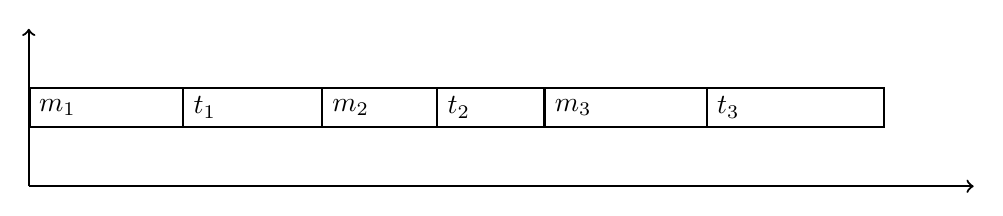
\begin{tikzpicture}[
  thick,
  myrect/.style={
    draw,
    rectangle split,
    rectangle split horizontal,
    rectangle split parts=#1,
    rectangle split part align=center
    } 
]

\node[myrect=6, anchor=west](assembly)
  {
  \nodepart[text width= 17mm]{one}$m_1$
  \nodepart[text width= 15mm]{two}$t_1$
  \nodepart[text width= 12mm]{three}$m_2$
  \nodepart[text width= 11mm]{four}$t_2$
  \nodepart[text width= 18mm]{five}$m_3$
  \nodepart[text width= 20mm]{six}$t_3$
  };
  
      % Draw axes
      \draw[thick,->] (0,-1) -- (0,1);
      \draw[thick,->] (0,-1) -- (12,-1);

\end{tikzpicture}

\end{document} 

  	% or use \input{mytikz}
  	\caption{The worst case assembly}
  	\label{fig:worst_case}
  \end{figure}
   \begin{figure}
   	\centering
   	\documentclass{standalone}
\usepackage{tikz}
\usetikzlibrary{calc, shapes, backgrounds}
\usepackage{standalone}
\usepackage{amsmath, amssymb}
\begin{document}

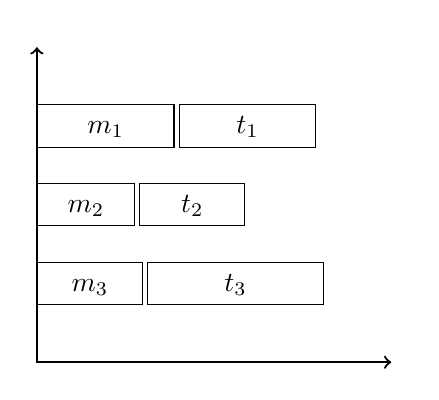
\begin{tikzpicture}
\tikzset{VertexStyle/.style = {anchor= west, draw, align= center, text height= 2.5mm}
}

    % Draw axes
    \draw [<->,thick] (0,4) node (yaxis) [above] {}
        |- (45mm,0) node (xaxis) [right] {};

   \node[VertexStyle, text width= 15mm] (rect1) at (0mm,3)  {$m_1$};
   \node[VertexStyle, text width= 15mm] (rect2) at (18mm,3) {$t_1$};
   
   \node[VertexStyle, text width= 10mm] (rect1) at (0mm,2)  {$m_2$};
   \node[VertexStyle, text width= 11mm] (rect2) at (13mm,2) {$t_2$};
      
   \node[VertexStyle, text width= 11mm] (rect1) at (0mm,1)  {$m_3$};
   \node[VertexStyle, text width= 20mm] (rect2) at (14mm,1) {$t_3$};
\end{tikzpicture}
\end{document} 

   	% or use \input{mytikz}
   	\caption{The best case assembly}
   	\label{fig:best_case}
   \end{figure}
 \newpage
 We can now start using $maxEnd$ and $minEnd$ to filter variables
  \begin{equation}\label{eq:lim_start_over}
  \begin{aligned}
 &(\forall t \in allTasks)\\
 &start(t) \le maxEnd-duration(t)
  \end{aligned}
  \end{equation}
   \begin{equation}\label{eq:lim_start_under}
  \begin{aligned}
 &(\forall t \in Tasks)\\
 &start(t) \ge minMoveDurs(t)
  \end{aligned}
  \end{equation}
 We set and upper bound for the start of a task by setting it to happen at latest the duration of the task time units before the $maxEnd$, since the task has to have time to execute before the end.
 
 To set a lower bound for the start of a task, we simply reason that the move to the task can start at its earliest at time 0. Therefore, we limit the task to start earliest direct after the minimum move duration to it.
 
 The difference between \ref{eq:lim_start_over} and \ref{eq:lim_start_under} is that the upper limit can be set for all sorts of tasks, even the start and goal tasks, but the lower limit cannot be set for start and goal tasks. This is simply because the start and goal tasks do not have any move times to them since they are source and sink nodes.
 
  \begin{equation}\label{eq:63}
  (\forall t \in tasks) \; moveStart(t) \le maxEnd-(duration(t)+minMoveDurs(t))
  \end{equation}
  In order to limit the move start to a task we use the same reasoning as with start. But now we have to account for that there comes a task after the move and a duration of the move itself. So we have to subtract the duration of the task and the duration of the move. Since we do not know the exact length of the move, we have to use the value we know the duration can not be lower than, which is $minMoveDuration$.
  
  \begin{equation}\label{eq:66}
  \begin{aligned}
  makeSpan &\le maxEnd \land\\
  makespan &\ge minEnd
  \end{aligned}
  \end{equation}
  We have already calculated the limits for the whole assembly, $maxEnd$ and $minEnd$. Now we just enforce them on the makespan.
  
  \begin{equation}
  \begin{aligned}\label{eq:67}
  &(\forall t \in tasks)\\
  &\begin{aligned}
  (\forall i \in \{0 , \ldots , maxMoveDurs(t)\} / \{&timeMatrix3D(task,j,k) :\\
  &\forall j \in tasks,\\
  &\begin{aligned}
  &\forall k \in \{1 , \ldots , timeMatrixDepth\}\\
  &t \neq j\})
  \end{aligned}
  \end{aligned}\\
  &moveDuration(t) \neq i
  \end{aligned}
  \end{equation}
 We know that the value for move duration will be one of the values in the time matrix, hence we can restrict the duration to only those values. We do that by coming up with the values that the duration cannot assume, and limits the duration to not have those values in its domain.
  
  \begin{equation}
  \begin{aligned}\label{eq:69}
  &(\forall t \in tasks / taking) \\
  &moveStart(t) \ge min(\{duration(tt) + minMoveDurs(tt) : \forall tt \in taking\})
  \end{aligned}
  \end{equation}
  The first thing that has to happen to a component in the assembly is that is has to be picked up. So since the assembly starts out with empty machines the first thing that has to happen, with the exception of a tool change, is a take task. Therefore, we can limit that start of the tasks not being take tasks to happen at earliest after the task with the smallest sum of duration and minimum move duration.
  
  \begin{equation}
  \begin{aligned}\label{eq:70}
  &(\forall t \in tasks)\\
  &\begin{aligned}
  prevTasks = \{task : &\forall task \in tasks,\\
  &componentCreated(task) \in componentsUsed(t)\},
  \end{aligned}\\
  &\begin{aligned}
  nbrMachines &\ge |prevTasks|,\\
  0 &< |prevTasks|,
  \end{aligned}\\
  &start(t) \ge max(\{duration(pt) + minMoveDurs(pt) : \forall pt \in prevTasks\}) \\
  \end{aligned}
  \end{equation}
  The start of a task can be even further limited by analysing the components used by the task and how that relates to what components are created by other tasks.
  
  Lets take task $t$ as an example. We start by getting all tasks that creates the components that is used in task $t$, $prevTasks$. These tasks has to come before task $t$ since the component that they create cannot be used before they are created. If the number of machines are greater than or equal to the number of task preceding task t, then the best scheduling that can be done is to do all tasks in parallel. That means that task $t$ can start at earliest after the one of the proceeding tasks taking the longest to complete.
  
  \begin{equation}
  \begin{aligned}\label{eq:71}
  &(\forall t \in tasks) \\
  &\begin{aligned}
  prevTasks = \{task : &\forall task \in tasks,\\
  &componentCreated(task) \in componentsUsed(t)\},
  \end{aligned} \\
  &nbrMachines < |prevTasks|,  \\
  &start(t) \ge \frac{\left(\sum_{\forall pt \in prevTasks}duration(pt) + minMoveDurs(pt)\right)}{nbrMachines}
  \end{aligned}
  \end{equation}
  But if the number of machines is fewer than the number of preceding tasks, the best we can do is divide them as equally as possible over the machines. This is the same reasoning as when we calculated $minEnd$ in equation \ref{eq:minEnd}.
  
  \begin{equation}\label{eq:72}
  \begin{aligned}
  &(\forall t \in tasks) \\
  &succTasks = \{task : \forall task \in tasks,\\
  &componentsUsed(t) \subset taskCompleteSubComponent(task), \\
  &componentsUsed(t) \cup taskCompleteSubComponents(task) \neq \emptyset\}, \\
  &\begin{aligned}
  nbrMachines &\ge |succTasks|,\\
  0 &< |succTasks|,
  \end{aligned}\\
  &\begin{aligned}
  start(t) \le maxEnd - max(\{&duration(st) + minMoveDurs(st) :\\
  &\forall st \in succTasks\}) - duration(t)
  \end{aligned}\\
  \end{aligned}
  \end{equation}
  To set the upper limit for the start of tasks we use a little bit different strategy.
  
  We know that if a component $c$ has been mounted on another component, $c$ cannot be used again on its own. Therefore, a task that uses component $c$ has to come before the tasks that uses a component in which $c$ is a part of.
  
  We use the same strategy as in \ref{eq:70} and look at the best case scenario where the tasks are performed concurrently on all machines. The difference here from \ref{eq:70} is that here we have to look at the maximum end of the assembly and subtract the successor task which takes the longest to perform and the duration of the task in question.
  
  \begin{equation}\label{eq:73}
  \begin{aligned}
  &(\forall t \in tasks)\\
  &succTasks = \{task : \forall task \in tasks, \\
  &componentsUsed(t) \subset taskCompleteSubComponent(task), \\
  &componentsUsed(t) \cup taskCompleteSubComponents(task) \neq \emptyset\}, \\
  &nbrMachines \le |succTasks|, \\
  &\begin{aligned}
  start(t) \; \le \; &maxEnd - \frac{\left(\sum_{\forall st \in succTasks}duration(st) + minMoveDurs(st)\right)}{nbrMachines}\\
  &- duration(t)
  \end{aligned}
  \end{aligned}
  \end{equation}
  As with \ref{eq:71} we look at the worst case scenario.
  
  
  \subsection{Predecessor filter}
  Since the predecessors are searched by the solver before searching the start variables, reducing their domains has potential to help reduce the total runtime considerably.
 
  \begin{equation}\label{eq:75}
  (\forall t1, \forall t2 \in taking) \; pred(t1) \neq t2
  \end{equation}
  \begin{equation}\label{eq:76}
  (\forall t1, \forall t2 \in putting \cup mounting) \; pred(t1) \neq t2
  \end{equation}
 In our model the tools can only pick up one component at a time. This also means that if a task puts down a component or mounts one, there cannot be a mount or put task directly afterwards.
  
  \begin{equation}
  \begin{aligned}\label{eq:78}
  &(\forall t \in tasks)\\
  &nonPredecessors = \{t_2 : \forall t_2 \in tasks, \\
  &componentsUsed(t) \subset taskCompleteSubComponents(t_2) \; \lor \\
  &componentsUsed(t) \subset subComponents(componentCreated(t_2))\} \\
  &(\forall nonPred \in nonPredecessors) \\
  &pred(t) \neq nonPred, \\
  \end{aligned}
  \end{equation}
  Using a similar reasoning as in \ref{eq:72} and \ref{eq:73}, we can find the tasks that cannot be the predecessor of task $t$. We look at what tasks uses the components that has the components used in $t$ as sub-components. This means that those components cannot come before task $t$, and therefore cannot be predecessors of $t$.
  
  \begin{equation}\label{eq:79}
  \begin{aligned}
  &(\forall startTask \in startTasks)\\
  &(\forall putTask \in putting)\\
  &pred(putTask) \neq startTask
  \end{aligned}
  \end{equation}
  \begin{equation}\label{eq:80}
   \begin{aligned}
   &(\forall startTask \in startTasks)\\
   &(\forall mountTask \in mounting)\\
   &pred(mountTask) \neq startTask 
   \end{aligned}
  \end{equation}
  As mentioned before, a component has to be picked up first before it can be manipulate in any way and the assembly has to start with a take task. Therefore, we can say that an assembly cannot start with neither a put task nor a mount task.
  
  The same could be said for move tasks, but since they need to be in an ordered group, a constraint like these would no make any difference.
  
  \begin{equation}\label{eq:81}
  \begin{aligned}
  &(\forall goalTask \in goalTasks) \\
  &(\forall takeTask \in taking) \\
  &pred(goalTask) \neq takeTask
  \end{aligned}
  \end{equation}
  The same way we can observe that an assemble needs to start with a take task, we can observe that an assembly cannot end with a take task. There is no component in the assembly that does not end up in the finished assembly, therefore the assembly cannot end with a machine holding a component, since it needs to be on the output in some way. 
  
  \begin{equation}
  \begin{aligned}\label{eq:82}
  &\begin{aligned}
  counts &= \{i : \forall task \in outputTasks, \; i \in \{0 , \ldots , 1\}\}, \\
  outputTasks &= \{task : \forall task \in tasks, \; output(task) > 0\}, \\
  goalPreds &= \{pred(task) : \forall task \in goalTasks\},
  \end{aligned} \\
  &global\_cardinality(goalPreds, \; outputTasks, \; counts) \; \land\\
  &\sum counts > 0
  \end{aligned}
  \end{equation}
   \begin{equation}
   \begin{aligned}\label{eq:83}
   &\begin{aligned}
   counts &= \{i : \forall task \in startTasks, \; i \in \{0 , \ldots , 1\}\}, \\
   takePreds &= \{pred(task) : \forall task \in taking\}, 
   \end{aligned}\\
   &global\_cardinality(takePreds, \; startTasks, \; counts) \; \land\\
   &\sum counts > 0
   \end{aligned}
   \end{equation}
 Continuing the reasoning around what tasks can come first and not we can expand with which tasks has to come last. We cannot limit the last task on each arm to be on an output, because it does not necessarily need to be that. Although, among the last tasks in the assembly there needs to be a task on an output. We can easily check that by placing a constraint over the $pred$ variables for the goal tasks. This is what \ref{eq:82} says.
 
 We can do the same reasoning with what needs to come first in the assembly. As we stated before, a take task has to be the first task in the assembly. And as with the last tasks in the assembly, the first task of a machine does not have to be a take task, but there needs to be at least one take task among the first tasks. We ensure this in \ref{eq:83} by placing a constraint over the $pred$ variables for the take tasks.
\chapter{Case Study}\label{cha:assembly}
In order to develop and test the model, we have chosen to focus on one case study. In this case study the robot is assembling an enclosed emergency stop button used in industrial environments[bild?]. This assembly is composed of 5 components; a top, a button, a ring, a switch and a bottom. The button needs to be inserted in the top and then the ring needs to be screwed onto the underside of the button in order to secure it to the top. The switch needs to be mounted in the bottom and lastly the top part, with button and ring, needs to be mounted on the bottom, with the switch. For a exploded-view of the assembly, see figure [??].

The assembly includes objects such as trays and fixtures. A tray is a holder where components reside until they are needed in the assembly. A fixture is a holder in which components can be put and another components can be mounted on it.

21 steps has been identified as steps needed for the assembly and they are taken from a video of an existing assembly created by hand. The steps are as follows:

\begin{description}
\item[Take top] Takes the top component from its tray

\item[Put top in fixture] Puts the taken top component and puts it in a fixture

\item[Take button] Takes the button component from its tray

\item[Mount button on top] Mounts the taken button component onto the top component in a fixture

\item[Angle top-button] Angles the assembly that is the top and button component, from here on called top-button

\item[Lift top-button, hold top button] Lifts the top-button by holding the button

\item[Lift top-button, support] Lifts the top-button by supporting the top from underneath

\item[Turn top-button] Turns the top-button by holding the button

\item[Take ring] Takes the ring from its tray

\item[Mount ring on top-button, hold] Mounts the ring on top-button by holding the button

\item[Mount ring on top-button, mount] Mounts the ring on the top-button holding and screwing the ring. The assembly created by the top-button and the ring is here on after called top-button-ring

\item[Fixate top-button-ring] Fixates the top-button ring using the side of a fixture in order to get it straight.

\item[Put top-button-ring in top tray] The top-button-ring is put in the top tray in order to put it away for a while and then to be picked up later.

\item[Take top-button-ring from top tray] Takes the top-button-ring from the top tray where it was previously put.

\item[Take bottom] Takes the bottom component from its tray.

\item[Put bottom in fixture] Puts the bottom component in a fixture.

\item[Take switch] Takes the switch component from its tray.

\item[Mount switch in bottom] Mounts the switch on the bottom in the fixture the bottom was put in. The created assembly created here will here on after be called bottom-switch.

\item[Take bottom-switch] Takes the created bottom-switch from the fixture it was created in.

\item[Put bottom-switch on table] Puts the bottom-switch on the table.

\item[Mount top-button-ring on bottom-switch] Mounts the top-button-ring on the button-switch on the table.
\end{description}

\noindent Most of the steps are self explanatory, but there are a few steps which are quite special that might need some more explanation. In steps \textbf{Mount ring on top-button, hold} and \textbf{Mount ring on top-button, mount} we have the button component put in the hole of the top and we need to secure it using the ring component. To do this we utilize something that is special for YuMi\textsuperscript\textregistered, we will use only the two arms in order to mount the ring. We will do it mid air with one arm holding the top-button by holding the button part, having it upside-down compared to how it was in the fixture, and with the other arm screwing the ring in place. In order to prepare for this, we start at the end of step \textbf{Mount button on top}, where we just created the assembly top-button, but the button is only loosely sitting in the hole of the top. We angle the assembly in task \textbf{Angle top-button} about 45$^\circ$ in order to create a gap under the assembly so the other arm can reach under the assembly and help lift it from the fixture in tasks \textbf{Lift top-button, support} and \textbf{Lift top-button, hold top button}. Finally we rotate the top-button by only holding it with one arm in the button part of the assembly and are now ready for the ring to be mounted.
It should be noted that since the operations of lifting the top-button and mounting the ring takes two arms and we have here split the operations into two tasks each, one for each arm, the tasks \textbf{Mount ring on top-button, hold} and \textbf{Mount ring on top-button, mount} needs to be performed at the same time. The same goes for  \textbf{Lift top-button, support} and \textbf{Lift top-button, hold top button}.

\begin{landscape}
\begin{figure}
\documentclass{standalone}
\usepackage{standalone}
\begin{document}
\tikzstyle{task} = [rectangle, minimum width=3cm, minimum height=1cm, text centered, draw=black]
\tikzstyle{arrow} = [thick,->,>=stealth]
\begin{tikzpicture}[node distance=2cm]
\node (1) [task] {Take top};
\node (2) [task, right of=1, xshift=2.5cm] {Put top in fixture};

\node (3) [task, below of=1] {Take button};
\node (4) [task, below of=2] {Mount button on top};

\node (5) [task, xshift=2.5cm, right of=4] {Angle top-button};

\node (6) [task, right of=5, xshift=3cm, yshift=1cm] {Lift top-button, hold};
\node (7) [task, below of=6] {Lift top-button, support};

\node (8) [task, right of=7, xshift=3.5cm, yshift=1cm] {Turn top-button};

\node (10) [task, below of=8] {Mount ring, hold};
\node (11) [task, below of=10] {Mount ring, mount};

\node (9) [task, below of=11] {Take ring};

\node (12) [task, left of=11, xshift=-4cm, yshift=1cm] {Fixate top-button-ring};

\node (13) [task, left of=12, xshift=-10cm] {Put top-button-ring in top tray};
\node (14) [task, below of=13] {Take top-button-ring from top tray};

\node (15) [task, below of=9, yshift=-1.5cm] {Take switch};
\node (16) [task, left of=15, xshift=-3cm] {Mount switch};

\node (17) [task, below of=15] {Take bottom};
\node (18) [task, below of=16] {Put button in fixture};

\node (19) [task, left of=16, xshift=-3.5cm] {Take button-switch};

\node (20) [task, left of=19, xshift=-5cm] {Put bottom-switch on table};

\node (21) [task, above of=20] {Mount top-button-ring on bottom-switch};

\draw [arrow] (1) -- (2);
\draw [arrow] (3) -- (4);
\draw [arrow] (2) -- (4);
\draw [arrow] (4) -- (5);
\draw [arrow] (5) -- (6);
\draw [arrow] (5) -- (7);
\draw [arrow] (7) -- (8);
\draw [arrow] (6) -- (8);
\draw [arrow] (8) -- (10);
\draw [arrow] (10) -- (12);
\draw [arrow] (9) -- (11);
\draw [arrow] (11) -- (12);
\draw [arrow] (12) -- (13);
\draw [arrow] (13) -- (14);
\draw [arrow] (15) -- (16);
\draw [arrow] (17) -- (18);
\draw [arrow] (18) -- (16);
\draw [arrow] (16) -- (19);
\draw [arrow] (19) -- (20);
\draw [arrow] (20) -- (21);
\draw [arrow] (14) -- (21);

\end{tikzpicture}
\end{document}
\caption{The case study assembly}
\end{figure}
\end{landscape}

%\documentclass{standalone}
\begin{document}
\begin{table}
\centering
\begin{tabular}{c|l|p{6cm}}
Step & Name                                  & Comment\\
\hline
1   & Take top                               & Takes the top component from its tray\\
2   & Put top in fixture                     & Puts the taken top component and puts it in a fixture\\
3   & Take button                            & Takes the button component from its tray\\
4   & Mount button on top                    & Mounts the taken button component onto the top component in a fixture\\
5   & Angle top-button                       & Angles the assembly that is the top and button component, from here on called top-button\\
6   & Lift top-button, hold top button       & Lifts the top-button by holding the button\\
7   & Lift top-button, support               & Lifts the top-button by supporting the top from underneath\\
8   & Turn top-button                        & Turns the top-button by holding the button\\
9   & Take ring                              & Takes the ring from its tray\\
10  & Mount ring on top-button, hold         & Mounts the ring on top-button by holding the button\\
11  & Mount ring on top-button, mount        & Mounts the ring on the top-button holding and screwing the ring. The assembly created by thetop-button and the ring is here on after called top-button-ring\\
12  & Fixate top-button-ring                 & Fixates the \\
13  & Put top-button-ring in top tray        &\\
14  & Take top-button-ring from top tray     &\\
15  & Take bottom                            &\\
16  & Put bottom in fixture                  &\\
17  & Take switch                            &\\
18  & Mount switch in bottom                 &\\
19  & Take bottom-switch                     &\\
20  & Put bottom-switch on table             &\\
21  & Mount top-button-ring on bottom-switch &\\
\end{tabular}
\caption{Steps in case study}\label{tab:assembly_steps}
\end{table}
\end{document}
\chapter{Evaluation}
The evaluation of the model

\section{The Setup}

\begin{tabular}{l|l}
Solver                    & Version \\ \hline
G12/FD                    & 1.6.0\\
JaCoP                     & 4.2 \\
Gecode                    & 4.3.2 \\
or-tools                  & Rev. 3782 \\
Opturion CPX              & 1.0.2 \\
\multirow{2}{*}{Chcoco 3} & Solver: 3.2.2 \\
                          & Parser: 3.2.0
\end{tabular}

\begin{landscape}
\hspace*{\fill}
\noindent\documentclass{standalone}
\begin{document}
\begin{tabular}{lc|c|c|c|c|c|c|c}
\multicolumn{9}{c}{G12} \\ 
\hline\hline Filter & \multicolumn{2}{c|}{Pred \& Dom} &\multicolumn{2}{c|}{Pred}  & \multicolumn{2}{c|}{Dom} & \multicolumn{2}{c}{None} \\ 
\hline Version & 1.6 & 2.0.1 & 1.6 & 2.0.1 & 1.6 & 2.0.1 & 1.6 & 2.0.1 \\ 
Time (ms)               & - & - & - & - & - & - & - & - \\ 
\# of integer variables & 174 & 292 & 174 & 313 & 154 & 269 & 154 & 290 \\ 
\# of boolean variables & 162 & 97 & 162 & 97 & 142 & 106 & 142 & 106 \\ 
\# of arrays            & 32 & 46 & 32 & 46 & 30 & 44 & 30 & 44 \\ 
\# of constraints       & 2555 & 584 & 1018 & 584 & 2248 & 558 & 711 & 558 \\ 
\% refeid               & 7.16\% & 15.92\% & 17.97\% & 15.92\% & 7.25\% & 17.02\% &22.92\% & 17.02\% \\ 
\end{tabular} 
\end{document}
\hspace*{\fill}
\\
\hspace*{\fill}
\documentclass{standalone}
\begin{document}
\begin{table}[H]
\footnotesize
\centering
\begin{tabular}{lc|c|c|c|c|c|c|c}
\multicolumn{9}{c}{JaCoP} \\ 
\hline\hline Filter & \multicolumn{2}{c|}{Pred \& Temp} &\multicolumn{2}{c|}{Pred}  & \multicolumn{2}{c|}{Temp} & \multicolumn{2}{c}{None} \\ 
\hline Version & 1.6 & 2.0.1 & 1.6 & 2.0.1 & 1.6 & 2.0.1 & 1.6 & 2.0.1 \\ 
Time (ms)               & 658 & - & 1011156 & - & - & - & - & - \\
Time                    & 0:00:00 & - & 0:16:51 & - & - & - & - & - \\ 
\# of integer variables & 129 & 225 & 129 & 246 & 129 & 230 & 129 & 251 \\ 
\# of boolean variables & 42 & 27 & 42 & 27 & 42 & 27 & 42 & 27 \\ 
\# of arrays            & 30 & 53 & 30 & 53 & 28 & 50 & 28 & 50 \\ 
\# of constraints       & 2195 & 429 & 741 & 429 & 1951 & 420 & 497 & 420 \\ 
\% refeid               & 2.87\% & 6.29\% & 8.50\% & 6.29\% & 3.22\% & 6.42\% & 12.67\% & 6.42\% \\ 
\end{tabular}
\caption{Results for JaCoP}
\end{table}
\end{document}
\hspace*{\fill}
\\
\hspace*{\fill}
\documentclass{standalone}
\begin{document}
\begin{table}[H]
\footnotesize
\centering
\begin{tabular}{lc|c|c|c|c|c|c|c}
\multicolumn{9}{c}{Gecode} \\ 
\hline\hline Filter & \multicolumn{2}{c|}{Pred \& Temp} &\multicolumn{2}{c|}{Pred}  & \multicolumn{2}{c|}{Temp} & \multicolumn{2}{c}{None} \\ 
\hline Version & 1.6 & 2.0.1 & 1.6 & 2.0.1 & 1.6 & 2.0.1 & 1.6 & 2.0.1 \\ 
Time (ms)               & - & 60 & - & 71761 & - & 99 & - & 70925 \\ 
Time                    & - & 0:00:00 & - & 0:01:11 & - & 0:00:00 & - & 0:01:10 \\ 
\# of integer variables & 129 & 225 & 129 & 246 & 129 & 230 & 129 & 251 \\ 
\# of boolean variables & 42 & 27 & 42 & 27 & 42 & 27 & 42 & 27 \\ 
\# of arrays            & 30 & 57 & 30 & 57 & 28 & 50 & 28 & 50 \\ 
\# of constraints       & 2193 & 425 & 739 & 425 & 1951 & 420 & 497 & 420 \\ 
\% refeid               & 2.87\% & 6.35\% & 8.52\% & 6.35\% & 3.22\% & 6.42\% & 12.67\% & 6.42\% \\ 
\end{tabular}
\caption{Results for Gecode}\label{tab:res_gecode}
\label{tab:res_gecode}
\end{table}
\end{document}
\hspace*{\fill}
\\
\hspace*{\fill}
\documentclass{standalone}
\begin{document}
\begin{tabular}{lc|c|c|c|c|c|c|c}
\multicolumn{9}{c}{or-tools} \\ 
\hline\hline Filter & \multicolumn{2}{c|}{Pred \& Dom} &\multicolumn{2}{c|}{Pred}  & \multicolumn{2}{c|}{Dom} & \multicolumn{2}{c}{None} \\ 
\hline Version & 1.6 & 2.0.1 & 1.6 & 2.0.1 & 1.6 & 2.0.1 & 1.6 & 2.0.1 \\ 
Time (ms)               & 257 & ! & 672 & ! & 564 & ! & 600 & ! \\ 
\# of integer variables & 129 & 223 & 129 & 244 & 129 & 229 & 129 & 250 \\ 
\# of boolean variables & 42 & 27 & 42 & 27 & 42 & 27 & 42 & 27 \\ 
\# of arrays            & 31 & 50 & 31 & 50 & 29 & 43 & 29 & 43 \\ 
\# of constraints       & 2316 & 421 & 779 & 421 & 2046 & 416 & 509 & 416 \\ 
\% refeid               & 2.72\% & 6.41\% & 8.08\% & 6.41\% & 3.07\% & 6.49\% & 12.37\% & 6.49\% \\ 
\end{tabular} 
\end{document}
\hspace*{\fill}
\\
\hspace*{\fill}
\documentclass{standalone}
\begin{document}
\begin{table}[H]
\footnotesize
\begin{tabular}{lc|c|c|c|c|c|c|c}
\multicolumn{9}{c}{Opturion CPX - no warm start} \\ 
\hline\hline Filter & \multicolumn{2}{c|}{Pred \& Dom} &\multicolumn{2}{c|}{Pred}  & \multicolumn{2}{c|}{Dom} & \multicolumn{2}{c}{None} \\ 
\hline Version & 1.6 & 2.0.1 & 1.6 & 2.0.1 & 1.6 & 2.0.1 & 1.6 & 2.0.1 \\ 
Time (ms)               & 25163591 & !       & -       & !       & 7332356 & !       & -       & !       \\ 
\# of integer variables & 28736    & 9530    & 28736   & 28875   & 28716   & 9507    & 28716   & 28852	  \\ 
\# of boolean variables & 57284    & 18654   & 57284   & 57322   & 57264   & 18702   & 57264   & 57370	  \\ 
\# of arrays            & 32       & 4694    & 32      & 14366   & 30      & 28209   & 30      & 14382	  \\ 
\# of constraints       & 102519   & 33021   & 100982  & 100675  & 102212  & 33024   & 100675  & 100678  \\ 
\% refeid               & 55.91\%  & 56.26\% & 56.76\% & 56.86\% & 56.06\% & 56.24\% & 56.92\% & 56.85\% \\ 
\end{tabular} 
\end{table}
\end{document}
\hspace*{\fill}
\\
\hspace*{\fill}
\input{Tables/results_cpx_ws}
\hspace*{\fill}
\\
\hspace*{\fill}
\documentclass{standalone}
\begin{document}
\begin{table}[H]
\footnotesize
\centering
\begin{tabular}{lc|c|c|c|c|c|c|c}
\multicolumn{9}{c}{Choco3} \\ 
\hline\hline Filter & \multicolumn{2}{c|}{Pred \& Temp} &\multicolumn{2}{c|}{Pred}  & \multicolumn{2}{c|}{Temp} & \multicolumn{2}{c}{None} \\ 
\hline Version & 1.6 & 2.0.1 & 1.6 & 2.0.1 & 1.6 & 2.0.1 & 1.6 & 2.0.1 \\ 
Time (ms)               & - & - & - & - & - & - & - & - \\ 
Time                    & - & - & - & - & - & - & - & - \\ 
\# of integer variables & 129 & 246 & 129 & 246 & 129 & 230 & 129 & 251 \\ 
\# of boolean variables & 42 & 27 & 42 & 27 & 42 & 27 & 42 & 27 \\ 
\# of arrays            & 30 & 57 & 30 & 57 & 28 & 50 & 28 & 50 \\ 
\# of constraints       & 2193 & 425 & 739 & 425 & 1951 & 420 & 497 & 420 \\ 
\% reifeid               & 2.87\% & 6.35\% & 8.52\% & 6.35\% & 3.22\% & 6.42\% & 12.67\% & 6.42\% \\ 
\end{tabular}
\caption{Results for Choco3}\label{tab:res_choco}
\end{table}
\end{document}
\hspace*{\fill}
\end{landscape}


\chapter{Discussion}\label{cha:discuss}
The discussion of the results

As mentioned, in 1.6 the filters increase the number of constraints quite a bit. But the number of reified constraints are decreasing by quite a lot as well. This seems to indicate that the filters does not introduce more reified constraints, which is good.

Decrease in constraints could be connected to the difference in number of constraint when applying filters in 1.6 vs 2.0.1.

in 2.0.1 temp filter adds no constraints, pred filter adds small amount -> hints of pruning instead of relying on the solver to prune

Concurrent tasks vs. en task med två maskiner.
Två tasks ger mer generella constraints, man kan säga att all tasks tar upp en maskin alltid och att man begränsar det med ett constraint att vissa måste ske samtidigt. Man kan ha constraintet att alla tasks kan ha en predecessor.
En task gör att man måste kunna säga att tasks kan ta upp till så många maskiner som finns tillgängliga -> fler constraints. Man måste kunna säga att en task ska kunna ha flera predecessors -> fler constraints.


\chapter{Conclusions} \label{cha:conc}
Through this thesis we can conclude that the presented model representing the problem as a Job Shop Problem works well and can produce a result that is as good as the handmade solution.

We can also conclude that when it comes to choosing solvers there can be a very large difference in the performance. It can range from not being able to solve a problem in 4 hours to solve it in under 100 milliseconds. The best performance was achieved by Gecode in 60 milliseconds using the 2.0.1 version of MiniZinc. This is promising result for the new version. Interestingly the 1.6 version of the same solver could not solve the problem in 4 hours. But although the 2.0.1 version performed remarkably well for Gecode, two of the solvers were not able to read the FlatZinc file produced by that version, more specifically Opturion CPX and or-tools.

We tested applying filters that reduced the domains of temporal variables and predecessor variables. Our tests showed that these filters can have an positive inpact on the runtime result, and thereby confirming the results of Vilím in \cite{VilimBartak2002Batch} \cite{Vilim2002Precedence} and \cite{VilimBartak2002Sequence}.

The analysis of the resulting FlatZinc files showed that there was no relation between the resulting FlatZinc file and the runtime of the solver. Moreover, we found no relation between the percentage of reified constraints and the runtime of the solver.


\section{Further work}

Since the result from the solver was not evaluated on physical robot it could be a suitable continuation to try out the result on an actual robot. It could show problems not seen in the result itself, such as collisions etc.
\\\\
In this thesis we present a set of filter constraints to reduce the domains of the variables. The tests performed compared the result of using the filters versus not using the filters. It is not necessarily the case that all filters are needed, and all filters do probably not perform equally well. Therefore it might be of interest to test the each individual filter for it self and compare the filters against each other to see which performs the best and take that experience to come up with further filters.
\\\\
Since MiniZinc does not have support for customized searches, customized searches are not doable in regular MiniZinc. But in \cite{Bjordal} they present a constraint-based local search solver that performs local search in order to improve the runtime. Although Ejenstam concludes that local search performs poorly on the data in that thesis, it might be worth looking into. In \cite{yuan_2013} they conclude that Large neighborhood Search in combination with Hybrid Harmony Search performed very well for instances of Flexible Job Shop Problem. To incorporate such a search in the solver of \cite{Bjordal} might be beneficial to models such as this.
\\\\
As mentioned, our ambition for this thesis was originally to be able to run Ejenstam's data on our model, but the extended search space prevented us from that. The testing when developing the model, and thereby the tests for the extension to be able to run Ejenstam's data, was performed only on JaCoP. But as we can see from the results, there are solvers that could perform better. Hence, there might be a possibility to solve Ejenstam's data using those solvers. If an incorporation of local search, as mentioned above, can be done, it would probably further the possibility to adapt the model to the data.
\\\\
As mentioned before, our model assumes that there are as many sets of all the tools defined as there are machines, so that each machine has its own set of tools. This simulates an ideal world where we have all the resources we want, when in fact we might be limited to a few sets of tools. To be able to do more realistic schedulings that considers the amount of tools available, there would need to be a considerable number of constraints added to the model and it might be worth looking into in future work.

\makebibliography{report}

\begin{appendices}
 \chapter{Extended Model}\label{app:ext_mod}
This appendix contains constraints that are included in the model, but not as essential for the assembly as the ones in chapter \ref{cha:model}.

\section{Predecessor filter}
\begin{equation}\label{eq:74}
  alldifferent(\{pred(t) : \forall t \in tasks\})
  \end{equation}
 The \texttt{circuit} constraint already sees to it that the predecessors of the tasks forms a circuit. This means that all the predecessors will take on different values. However, we apply this \texttt{alldifferent} constraint in order to help the \texttt{circuit} make the predecessor variables take on different values.

 \begin{equation}
  \begin{aligned}\label{eq:85}
  (\forall comp &\in components) \\
  (\forall mountTask &\in mounting(comp)) \\
  (\forall takeTask &\in taking(comp)) \\
  pred(takeTask) &\neq mountTask
  \end{aligned}
  \end{equation}
  For all the tasks that operate on the same component we can restrict so the mount task of the component cannot be the predecessor of the take task. 
  
  \begin{equation}
  \begin{aligned}\label{eq:86}
  (\forall comp &\in components) \\
  (\forall putTask &\in putting{comp}, \; tray(putTask) > 0) \\
  (\forall takeTask &\in taking(comp), \; tray(putTask) = tray(takeTask)) \\
  pred(putTask) &\neq takeTask
  \end{aligned}
  \end{equation}
  We can also restrict the predecessor of a put task for a component to not be the take task for that component, if the two tasks are performed on the same tray. This can help in a situation when we want the assembly to put down a part for a moment and pick it up later, because if the part does not come in the tray from the beginning, i.e. it is not the component tray, we first need to put it in the tray before we are able to take it. 
  
  \begin{equation}
  \begin{aligned}\label{eq:87}
  (\forall f &\in fixtures) \\
  (\forall putTask &\in putting{comp}, \; fixture(putTask) = f) \\
  (\forall takeTask &\in taking(comp), \; fixture(takeTask) = f,\\
  &componentsUsed(putTask) \subset taskSubComponents(takeTask))\\
  pred(putTask) &\neq takeTask
  \end{aligned}
  \end{equation}
  As with constraint \ref{eq:99}, but we limit the predecessors instead.
  
  \begin{equation}
  \begin{aligned}\label{eq:88}
  (\forall group &\in \{1 , \ldots , nbrConcurrentGroups\}) \\
  (\forall t_1 &\in concurrentTasks(group)) \\
  (\forall t_2 &\in concurrentTasks(group) / \{t_1\}) \\
  pred(t_1) &\neq t_2 \land pred(t_2) \neq t_1
  \end{aligned}
  \end{equation}
  Since concurrent tasks need to happen simultaneously on different machines, they cannot be the predecessor to each other.
  
  \begin{equation}
  \begin{aligned}\label{eq:89}
  (\forall t_1 &\in tasks, \; componentCreated(t_1) > 0) \\
  (\forall t_2 &\in tasks, \; componentCreated(t_1) \in componentUsed(t_2)) \\
  pred(t_1) &\neq t_2
  \end{aligned}
  \end{equation}
 Sub-assembly components can only be used after they are created. Therefore, we can say that a task that uses a component created at task $t$ cannot be the predecessor of task $t$.
  
  \begin{equation}
  \begin{aligned}\label{eq:90}
  &(\forall precTask \in tasks) \\
  &(\forall t \in tasks, \; precTask \neq t,\\
  &\begin{aligned}componentUsed(precTask) \cup taskCompleteSubComponent(t) \subset\\
  taskCompleteSubComponents(t), \end{aligned}\\
  &componentsUsed(precTask) \cup taskCompleteSubComponents(t) \neq \emptyset \\
  &pred(precTask) \neq t
  \end{aligned}
  \end{equation}
 As in \ref{eq:103}, tasks has to be performed before the tasks having the component in the task as sub-component. This means the task cannot have any of these tasks as predecessor.
  
  \begin{equation}
  \begin{aligned}\label{eq:91}
  (\forall concGroup &\in concurrentTasks, \; |concGroup| = nbrMachines) \\
  concComps &= \bigcup_{\forall i \in concGroup}componentsUsed(i), \\
  concSubComps &= \bigcup_{\forall i \in concGroup}taskCompleteSubComponents(i), \\
  postTasks &= \{postTask : \forall postTask \in tasks,\\
  &concComps \cap taskCompleteSubComponents(postTask) \neq \emptyset\}\\
  preTasks &= \{preTask : \forall preTask \in tasks,\\
  &componentsUsed(preTask) \cap concSubComps \neq \emptyset\}, \\
  (\forall postTask &\in postTasks) \\
  (\forall predTask &\in preTasks) \\
  pred(postTask) &\neq preTask
  \end{aligned}
  \end{equation}
  If there is a group of concurrently executing tasks that take up all machines available they will act as a wall between the tasks before and after the group. It is guaranteed that the tasks after the group cannot have the tasks before the group as predecessors. We can extract the tasks before and after the concurrent tasks by analysing the components used, since the components used in the concurrent tasks will have the components used before as sub-components.
 
\input{Appendices/assembly_example}
\chapter{File \& Tool Manuals}\label{app:tool_manuals}
The data and tools used in this thesis are available for free to download and use at \url{https://github.com/Arclights/Thesis-Tools}. In this section we will describe the tools and data. All the tools are written in Java and are run using the \texttt{java -jar} command.

\section{File Formats}
There are two files used to produce the data for the solvers; it is the XML file that describes the assembly, and the time matrix file that describes the time it takes an arm to move between two tasks. For complete versions of the files used in the thesis see the link above.
\subsection{Assembly XML}\label{sec:xml}
In order to more easily create the data needed by the solvers, we created an XML format that that is more easy to deal with, that later is translated into MiniZinc code. For an outline of the XML format see listing \ref{list:xml}. Note that although it contain the basic parts, it is not a legit assembly XML file as it is not complete.

All ids must be unique within the area they are used. So for example there can only be one tray called "tray1", but there could be a fixture called "tray1" as well, but that would be bad practice since it would be confusing. Ids used must also be declared before they are used again. For example a component must be declared through a \texttt{Component} tag before being referenced to in a task. The number of declarations can theoretically be infinite, but since everything will be represented by integers in the model we are practically limited to the limit of integers.

The \texttt{Output} tag, \texttt{Tray} tag and \texttt{Fixture} tag defines an output, a tray and a fixture respectively. The \texttt{Component} tag defines a component. All components used in the assembly needs to be defined, including the sub assemblies, since we treat sub assemblies as components in our model. We also describe what components make up a subcomponent using the \texttt{SubComponent} tag, it can both be regular components or sub assemblies.

To define tools we use the \texttt{tool} tag and to define machines we use the \texttt{Machine tag}

To define a task we use the \texttt{Task} tag. Together with the id we specify the length of the task in some time unit. Inside the tag we declare the properties of the task. If the task is performed in a tray, we specify the tray used. The same goes for fixture. Only one of them can be declared at a time, since we cannot be at a tray and a fixture at the same time. We specify which components are used in the task. There can be multiple components associated with a task, but it is limited by the number of machines available. Although the translation program does not check whether or not this limit is exceeded. If there is a component created at the task we specify if by the \texttt{ComponentCreated} tag. There can only be a most one component created per task and can only occur in tasks where the action is mounting, but this is not checked by the translator either. If there is a particular tool needed for the task we specify it with the \texttt{ToolNeeded} tag. We specify what kind of action a task is using the \texttt{Action} tag.

To define a set of tasks that comes in an ordered group we use the \texttt{OrderedGroup} tag. The order of them listed in the XML file is the order in which they will be scheduled. There can be multiple ordered groups specified.

To define a set of task that needs to be performed concurrently we use the \texttt{ConcurrentGroup} tag. The order in the XML does not matter.

To define a set of tasks out of range of a machine we use the \texttt{TasksOutOfRange} tag. The id is the id of the machine that the tasks are out of range for. This is not declaring the machine, so it needs to be defined previously.

To define the tool change durations we use the \texttt{ToolChangeDurations} tag and for each tool change we want to define we use the \texttt{Change} tag. And we supply the tool we are changing from, the tool we are changing to and the duration it takes to perform.

\begin{figure}
\lstinputlisting[label=list:xml,captionpos=b,caption=The basic parts of the assembly XML. This is not a legit assembly file.,tabsize=3,frame=L,basicstyle=\footnotesize\ttfamily]{Listings/assembly.xml}
\end{figure}

\subsection{Time Matrix}\label{sec:time_matrix}
To supply the time it takes to move between the tasks we provide a time matrix using a time matrix. A row represents the task we are going from and the column represents the task we are going to. There are as many columns as there are tasks in the XML file, but there are one more rows than there are columns. This is to account for the starting position of the machines.

The file format is a comma separated values file (CSV). To identify which row and column belongs to the correct task, each row and column starts with the corresponding id from the XML file. The row for the start task must be named \emph{Start}. The times from every task to the place where the tools are changed and vice versa needs to be included as a column and a row with the name \emph{Change tool}. The order in which the ids comes in the row and columns has to be the same. The file needs to be separated with semicolons in order to allow for commas in the ids. This means that the ids used in the assembly cannot have semicolons in them. The values for the times can be decimal values, they will be rounded of after the calculations by the translator. Figure \ref{fig:time_matrix} shows an example of the structure of the time matrix.

\begin{figure}[h]
\begin{tabular}{c|c|c|c|c}
& Take top & Put top in fixture & \dots & Mount button on top\\\hline
Start & 3 & 7 & \dots & 7\\\hline
Take top & 0 & 8 & \dots & 8\\\hline
Put top in fixture & 8 & 0 & \dots & 0\\\hline
$\vdots$ & $\vdots$ & $\vdots$ & $\ddots$ & $\vdots$\\\hline
Mount button on top & 8 & 0 & \dots & 0
\end{tabular}
\caption{Example of time matrix structure}
\label{fig:time_matrix}
\end{figure}

\section{AssemblyConv}\label{sec:assemblyConv}
\texttt{AssemblyConv} is the program used to convert the XML file and the time matrix file into data for the solver. It takes the matrix file and the XML as arguments and produces a MiniZinc file. For a detailed description of the syntax run the program without parameters.

\section{SchedPrinter}
\texttt{SchedPrinter} is used for visualising the outputted assembly from the solvers. It creates a Gant diagram in ASCII and outputs it to the screen. To get it to a file one can simply pipe it to one and it can then be shown in a regular text editor. But make sure that text wrapping is turned of as it will interfere with the visualisation. It takes a text file containing the output from the solver. This can easily be obtained by piping the output from a solver into a file. The program also takes an argument whether the text file provided is in the format that the JaCoP solver provides or the format G12 provides. The solvers using the G12 format is G12/FD, Gecode and or-tools, and the solvers using the JaCoP format is JaCoP and Choco3. The output format for Opturion CPX is nknown since we have not been able to run the model on it. When printing from the JaCoP format, the user has to supply the \texttt{.dzn} file so the printer can know the name of the tasks. For a detailed description of the syntax run the program without parameters or with \texttt{-h} as parameter. The output of the tasks with duration 0 will look weird, but that is because we cannot fit any characters in a box with a width of 0.

\section{FZNstat}
To obtain the statistics used in chapter \ref{cha:eval} we use \texttt{FZNstat}. The program does not take any parameters but will go over all the \texttt{.fzn} files in the directory it is run in and produce a result file for each of the \texttt{.fzn} files. The names of the result files are the same as the \texttt{.fzn} files but with \texttt{\_stat} at the end. So for example \texttt{jacop.fzn} will get the result file \texttt{jacop\_stat}. The result files will contain a little bit more information about individual constraints than what was presented in chapter \ref{cha:eval}.
\end{appendices}
\end{document} 
